\documentclass[11pt,a4paper]{article}
\usepackage[T1]{fontenc}
\usepackage[utf8]{inputenc}
\usepackage[turkish,shorthands=off]{babel}
\usepackage{amsmath,amsthm}
\usepackage{newtxtext,newtxmath}
\usepackage[margin=25mm]{geometry}
\usepackage{setspace}
\onehalfspacing
\usepackage[mathlines]{lineno}
\linenumbers
\usepackage{graphicx}
\usepackage{booktabs}
\usepackage{longtable}
\usepackage[section]{placeins}
\makeatletter
\newcommand{\rawinput}[1]{\@@input #1 }
\makeatother
\usepackage{multirow}
\usepackage{algorithm}
\usepackage[noend]{algpseudocode}
\usepackage{xcolor}
\usepackage[round,authoryear]{natbib}
\usepackage{xurl}
\usepackage[hidelinks]{hyperref}
\usepackage{nameref}
\usepackage{siunitx}
\sisetup{group-separator={,},group-minimum-digits=4}
\usepackage[labelfont=bf,labelsep=space]{caption}
\captionsetup[figure]{name=Şekil}
\setlength{\emergencystretch}{2em}
\setcounter{secnumdepth}{0}
\newtheorem{lemma}{Lemma}
\newtheorem{proposition}{Proposition}
% generated by paper2/experiments/make_numbers.py; do not edit by hand
\newcommand{\AblEqualSplitAll}{+1.90}
\newcommand{\AblEqualSplitLit}{+4.12}
\newcommand{\AblEqualSplitLitBeats}{19}
\newcommand{\AblEqualSplitMtsplib}{+0.00}
\newcommand{\AblEqualSplitMtsplibBeats}{25}
\newcommand{\AblEqualSplitOrchard}{+1.06}
\newcommand{\AblEqualSplitOrchardBeats}{23}
\newcommand{\AblEqualSplitOsm}{+1.34}
\newcommand{\AblEqualSplitOsmBeats}{21}
\newcommand{\AblEqualSplitVlsi}{+5.54}
\newcommand{\AblEqualSplitVlsiBeats}{12}
\newcommand{\AblGeNolsAll}{+1.06}
\newcommand{\AblGeNolsLit}{+1.62}
\newcommand{\AblGeNolsLitBeats}{12}
\newcommand{\AblGeNolsMtsplib}{+1.20}
\newcommand{\AblGeNolsMtsplibBeats}{31}
\newcommand{\AblGeNolsOrchard}{+1.35}
\newcommand{\AblGeNolsOrchardBeats}{27}
\newcommand{\AblGeNolsOsm}{-0.17}
\newcommand{\AblGeNolsOsmBeats}{56}
\newcommand{\AblGeNolsVlsi}{+1.67}
\newcommand{\AblGeNolsVlsiBeats}{12}
\newcommand{\AblKmeansBalAll}{+8.30}
\newcommand{\AblKmeansBalLit}{+5.78}
\newcommand{\AblKmeansBalLitBeats}{6}
\newcommand{\AblKmeansBalMtsplib}{+2.70}
\newcommand{\AblKmeansBalMtsplibBeats}{25}
\newcommand{\AblKmeansBalOrchard}{+11.67}
\newcommand{\AblKmeansBalOrchardBeats}{0}
\newcommand{\AblKmeansBalOsm}{+13.61}
\newcommand{\AblKmeansBalOsmBeats}{0}
\newcommand{\AblKmeansBalVlsi}{+7.48}
\newcommand{\AblKmeansBalVlsiBeats}{4}
\newcommand{\AblKmeansTspAll}{+22.87}
\newcommand{\AblKmeansTspLit}{+20.56}
\newcommand{\AblKmeansTspLitBeats}{0}
\newcommand{\AblKmeansTspMtsplib}{+13.03}
\newcommand{\AblKmeansTspMtsplibBeats}{6}
\newcommand{\AblKmeansTspOrchard}{+26.03}
\newcommand{\AblKmeansTspOrchardBeats}{0}
\newcommand{\AblKmeansTspOsm}{+26.44}
\newcommand{\AblKmeansTspOsmBeats}{0}
\newcommand{\AblKmeansTspVlsi}{+20.49}
\newcommand{\AblKmeansTspVlsiBeats}{0}
\newcommand{\AblNnTourAll}{+0.50}
\newcommand{\AblNnTourLit}{+0.13}
\newcommand{\AblNnTourLitBeats}{33}
\newcommand{\AblNnTourMtsplib}{+0.25}
\newcommand{\AblNnTourMtsplibBeats}{38}
\newcommand{\AblNnTourOrchard}{+0.75}
\newcommand{\AblNnTourOrchardBeats}{33}
\newcommand{\AblNnTourOsm}{+0.63}
\newcommand{\AblNnTourOsmBeats}{31}
\newcommand{\AblNnTourVlsi}{+1.11}
\newcommand{\AblNnTourVlsiBeats}{25}
\newcommand{\AblNoBalanceAll}{+2.08}
\newcommand{\AblNoBalanceLit}{+2.58}
\newcommand{\AblNoBalanceLitBeats}{0}
\newcommand{\AblNoBalanceMtsplib}{+2.70}
\newcommand{\AblNoBalanceMtsplibBeats}{0}
\newcommand{\AblNoBalanceOrchard}{+1.82}
\newcommand{\AblNoBalanceOrchardBeats}{0}
\newcommand{\AblNoBalanceOsm}{+2.31}
\newcommand{\AblNoBalanceOsmBeats}{0}
\newcommand{\AblNoBalanceVlsi}{+1.68}
\newcommand{\AblNoBalanceVlsiBeats}{0}
\newcommand{\AblNoPolishAll}{+2.57}
\newcommand{\AblNoPolishLit}{+2.76}
\newcommand{\AblNoPolishLitBeats}{0}
\newcommand{\AblNoPolishMtsplib}{+4.25}
\newcommand{\AblNoPolishMtsplibBeats}{0}
\newcommand{\AblNoPolishOrchard}{+2.28}
\newcommand{\AblNoPolishOrchardBeats}{0}
\newcommand{\AblNoPolishOsm}{+2.43}
\newcommand{\AblNoPolishOsmBeats}{0}
\newcommand{\AblNoPolishVlsi}{+1.84}
\newcommand{\AblNoPolishVlsiBeats}{0}
\newcommand{\AblSweepTspAll}{+3.60}
\newcommand{\AblSweepTspLit}{+3.68}
\newcommand{\AblSweepTspLitBeats}{21}
\newcommand{\AblSweepTspMtsplib}{+1.55}
\newcommand{\AblSweepTspMtsplibBeats}{38}
\newcommand{\AblSweepTspOrchard}{+0.09}
\newcommand{\AblSweepTspOrchardBeats}{44}
\newcommand{\AblSweepTspOsm}{+6.37}
\newcommand{\AblSweepTspOsmBeats}{4}
\newcommand{\AblSweepTspVlsi}{+6.30}
\newcommand{\AblSweepTspVlsiBeats}{4}
\newcommand{\CountLarge}{39}
\newcommand{\CountMid}{54}
\newcommand{\CountSmall}{43}
\newcommand{\DefFinalLarge}{\ensuremath{\infty}}
\newcommand{\DefFinalMid}{242.8}
\newcommand{\DefFinalSmall}{3.2}
\newcommand{\HgFirstGreedyFruit}{-0.1}
\newcommand{\HgFirstGreedyRel}{+5.2}
\newcommand{\HgFirstGreedyWin}{100}
\newcommand{\HgFirstKdFruit}{+0.5}
\newcommand{\HgFirstKdRel}{+13.2}
\newcommand{\HgFirstKdWin}{100}
\newcommand{\HgFirstKdstealFruit}{+0.4}
\newcommand{\HgFirstKdstealRel}{+4.7}
\newcommand{\HgFirstKdstealWin}{96}
\newcommand{\HgFirstOrtoolsOneFruit}{+0.0}
\newcommand{\HgFirstOrtoolsOneRel}{+1.3}
\newcommand{\HgFirstOrtoolsOneWin}{72}
\newcommand{\HgFirstRowblockFruit}{+1.1}
\newcommand{\HgFirstRowblockRel}{+8.0}
\newcommand{\HgFirstRowblockWin}{96}
\newcommand{\HgFrameAxisZero}{+12.0}
\newcommand{\HgFrameAxisZeroAbs}{12.0}
\newcommand{\HgFrameAxisZeroMax}{+31.3}
\newcommand{\HgFrameOracle}{-0.3}
\newcommand{\HgFrameOracleAbs}{0.3}
\newcommand{\HgFrameOracleMax}{+10.5}
\newcommand{\HgFramePsbAxisZero}{+11.9}
\newcommand{\HgFramePsbAxisZeroAbs}{11.9}
\newcommand{\HgFramePsbAxisZeroMax}{+38.6}
\newcommand{\HgGreedyRec}{+0.1}
\newcommand{\HgGreedyRel}{+7.3}
\newcommand{\HgGreedyRelMax}{+34.8}
\newcommand{\HgGreedyRelMin}{-13.6}
\newcommand{\HgKMax}{33}
\newcommand{\HgKMin}{4}
\newcommand{\HgKdPlanMs}{0.13}
\newcommand{\HgKdRec}{-0.3}
\newcommand{\HgKdRel}{+20.5}
\newcommand{\HgKdRelMax}{+53.6}
\newcommand{\HgKdRelMin}{-6.7}
\newcommand{\HgKdstealRec}{-0.3}
\newcommand{\HgKdstealRel}{+8.9}
\newcommand{\HgKdstealRelMax}{+44.8}
\newcommand{\HgKdstealRelMin}{-10.5}
\newcommand{\HgN}{50}
\newcommand{\HgOrtoolsOneRec}{-0.0}
\newcommand{\HgOrtoolsOneRel}{+2.0}
\newcommand{\HgOrtoolsOneRelMax}{+19.5}
\newcommand{\HgOrtoolsOneRelMin}{-13.8}
\newcommand{\HgPGreedy}{2.1e-09}
\newcommand{\HgPKd}{5.9e-14}
\newcommand{\HgPKdsteal}{2.8e-10}
\newcommand{\HgPOrtoolsOne}{6.5e-03}
\newcommand{\HgPRowblock}{5.1e-03}
\newcommand{\HgPlanMs}{1.86}
\newcommand{\HgPrecision}{88.3}
\newcommand{\HgPsbPlanMs}{2}
\newcommand{\HgPsbRec}{+0.0}
\newcommand{\HgPsbRel}{+0.0}
\newcommand{\HgPsbRelMax}{+0.0}
\newcommand{\HgPsbRelMin}{+0.0}
\newcommand{\HgRecall}{67.8}
\newcommand{\HgRowblockRec}{-0.8}
\newcommand{\HgRowblockRel}{+3.0}
\newcommand{\HgRowblockRelMax}{+36.6}
\newcommand{\HgRowblockRelMin}{-23.0}
\newcommand{\HgRuns}{50}
\newcommand{\HgSparseGreedyFruit}{-0.1}
\newcommand{\HgSparseGreedyRel}{+9.4}
\newcommand{\HgSparseGreedyWin}{88}
\newcommand{\HgSparseKdFruit}{+0.5}
\newcommand{\HgSparseKdRel}{+27.9}
\newcommand{\HgSparseKdWin}{92}
\newcommand{\HgSparseKdstealFruit}{+0.4}
\newcommand{\HgSparseKdstealRel}{+13.1}
\newcommand{\HgSparseKdstealWin}{76}
\newcommand{\HgSparseOrtoolsOneFruit}{+0.0}
\newcommand{\HgSparseOrtoolsOneRel}{+2.8}
\newcommand{\HgSparseOrtoolsOneWin}{60}
\newcommand{\HgSparseRowblockFruit}{+1.3}
\newcommand{\HgSparseRowblockRel}{-2.0}
\newcommand{\HgSparseRowblockWin}{28}
\newcommand{\HgStealsMed}{3}
\newcommand{\HgTakeoverGain}{9.0}
\newcommand{\HgTakeoverP}{1e-12}
\newcommand{\HgTakeoverWin}{92}
\newcommand{\HgThetaErrMax}{0.34}
\newcommand{\HgThetaErrMed}{0.05}
\newcommand{\HgTreesMax}{3007}
\newcommand{\HgTreesMin}{444}
\newcommand{\HgWinGreedy}{94}
\newcommand{\HgWinKd}{96}
\newcommand{\HgWinKdsteal}{86}
\newcommand{\HgWinOrtoolsOne}{66}
\newcommand{\HgWinRowblock}{62}
\newcommand{\HgsMaxGreedy}{+10.9}
\newcommand{\HgsMaxKd}{+17.2}
\newcommand{\HgsMaxKdsteal}{+11.6}
\newcommand{\HgsMaxRowblock}{+15.6}
\newcommand{\HgsMinGreedy}{+1.6}
\newcommand{\HgsMinKd}{-0.0}
\newcommand{\HgsMinKdsteal}{-3.0}
\newcommand{\HgsMinRowblock}{-2.0}
\newcommand{\HsMaxGreedy}{+8.8}
\newcommand{\HsMaxOrtoolsOne}{+5.4}
\newcommand{\HsMaxRowblock}{+15.5}
\newcommand{\HsMaxStatic}{+9.7}
\newcommand{\HsMinGreedy}{-1.2}
\newcommand{\HsMinOrtoolsOne}{-1.2}
\newcommand{\HsMinRowblock}{+2.3}
\newcommand{\HsMinStatic}{+0.5}
\newcommand{\HsSettings}{17}
\newcommand{\HvGreedyRecallDiff}{+0.0}
\newcommand{\HvGreedyRelMax}{+34.4}
\newcommand{\HvGreedyRelMean}{+7.5}
\newcommand{\HvGreedyRelMin}{-4.8}
\newcommand{\HvGreedyRuns}{40}
\newcommand{\HvLatOsmOnehaNineZeroZero}{+133.2}
\newcommand{\HvLatOsmOnehaSixZero}{+0.2}
\newcommand{\HvLatOsmOnehaThreeZeroZero}{+13.8}
\newcommand{\HvLatOsmThreehaNineZeroZero}{+517.9}
\newcommand{\HvLatOsmThreehaSixZero}{+5.2}
\newcommand{\HvLatOsmThreehaThreeZeroZero}{+185.8}
\newcommand{\HvLatOsmTwohaNineZeroZero}{+341.6}
\newcommand{\HvLatOsmTwohaSixZero}{+0.4}
\newcommand{\HvLatOsmTwohaThreeZeroZero}{+72.4}
\newcommand{\HvLatSynOnehaNineZeroZero}{+244.9}
\newcommand{\HvLatSynOnehaSixZero}{-0.0}
\newcommand{\HvLatSynOnehaThreeZeroZero}{+24.2}
\newcommand{\HvOrtoolsOneRecallDiff}{+0.1}
\newcommand{\HvOrtoolsOneRelMax}{+15.9}
\newcommand{\HvOrtoolsOneRelMean}{+2.7}
\newcommand{\HvOrtoolsOneRelMin}{-9.1}
\newcommand{\HvOrtoolsOneRuns}{40}
\newcommand{\HvOrtoolsOneZeroRecallDiff}{+0.0}
\newcommand{\HvOrtoolsOneZeroRelMax}{+11.2}
\newcommand{\HvOrtoolsOneZeroRelMean}{+0.7}
\newcommand{\HvOrtoolsOneZeroRelMin}{-11.7}
\newcommand{\HvOrtoolsOneZeroRuns}{20}
\newcommand{\HvPGreedy}{1.4e-09}
\newcommand{\HvPOrtoolsOne}{2.4e-03}
\newcommand{\HvPRowblock}{6.3e-05}
\newcommand{\HvPStatic}{4.3e-04}
\newcommand{\HvPrecision}{88.3}
\newcommand{\HvPsbLnsOneRecallDiff}{+0.0}
\newcommand{\HvPsbLnsOneRelMax}{+22.7}
\newcommand{\HvPsbLnsOneRelMean}{-0.1}
\newcommand{\HvPsbLnsOneRelMin}{-13.8}
\newcommand{\HvPsbLnsOneRuns}{40}
\newcommand{\HvPsbPlanMs}{23}
\newcommand{\HvPsbRecallDiff}{+0.0}
\newcommand{\HvPsbRelMax}{+0.0}
\newcommand{\HvPsbRelMean}{+0.0}
\newcommand{\HvPsbRelMin}{+0.0}
\newcommand{\HvPsbRuns}{40}
\newcommand{\HvRecall}{68.0}
\newcommand{\HvReplanGapMin}{5.8}
\newcommand{\HvRowblockRecallDiff}{-0.8}
\newcommand{\HvRowblockRelMax}{+15.0}
\newcommand{\HvRowblockRelMean}{+3.4}
\newcommand{\HvRowblockRelMin}{-19.0}
\newcommand{\HvRowblockRuns}{40}
\newcommand{\HvStaticRecallDiff}{-1.0}
\newcommand{\HvStaticRelMax}{+16.4}
\newcommand{\HvStaticRelMean}{+2.7}
\newcommand{\HvStaticRelMin}{-9.0}
\newcommand{\HvStaticRuns}{40}
\newcommand{\HvTripsMed}{64}
\newcommand{\HvWinGreedy}{88}
\newcommand{\HvWinOrtoolsOne}{68}
\newcommand{\HvWinRowblock}{78}
\newcommand{\HvWinStatic}{70}
\newcommand{\InstAll}{136}
\newcommand{\LbGapMtsp}{17.1}
\newcommand{\LbGapOrch}{11.7}
\newcommand{\LbGapVlsi}{30.9}
\newcommand{\LitColumns}{12}
\newcommand{\LitCount}{52}
\newcommand{\LitFewKCount}{26}
\newcommand{\LitFewKHgaCount}{26}
\newcommand{\LitFewKHgaFinal}{10.1}
\newcommand{\LitFewKHsnrCount}{26}
\newcommand{\LitFewKHsnrFinal}{11.8}
\newcommand{\LitFewKMaCount}{26}
\newcommand{\LitFewKMaFinal}{8.9}
\newcommand{\LitFewKMilsCount}{26}
\newcommand{\LitFewKMilsFinal}{1.7}
\newcommand{\LitFewKPsbBeatsHga}{16}
\newcommand{\LitFewKPsbBeatsHsnr}{22}
\newcommand{\LitFewKPsbBeatsMa}{15}
\newcommand{\LitFewKPsbBeatsMils}{4}
\newcommand{\LitFewKPsbBeatsTuned}{14}
\newcommand{\LitFewKPsbBeatsWarm}{7}
\newcommand{\LitFewKPsbFinal}{5.9}
\newcommand{\LitFewKPsbTiesHga}{0}
\newcommand{\LitFewKPsbTiesHsnr}{0}
\newcommand{\LitFewKPsbTiesMa}{0}
\newcommand{\LitFewKPsbTiesMils}{0}
\newcommand{\LitFewKPsbTiesTuned}{0}
\newcommand{\LitFewKPsbTiesWarm}{0}
\newcommand{\LitFewKTunedCount}{26}
\newcommand{\LitFewKTunedFinal}{6.2}
\newcommand{\LitFewKWarmCount}{26}
\newcommand{\LitFewKWarmFinal}{4.0}
\newcommand{\LitLCount}{36}
\newcommand{\LitLHgaFinal}{13.4}
\newcommand{\LitLHgaOne}{\ensuremath{\infty}}
\newcommand{\LitLHgaTen}{\ensuremath{\infty}}
\newcommand{\LitLHsnrFinal}{15.3}
\newcommand{\LitLHsnrOne}{\ensuremath{\infty}}
\newcommand{\LitLHsnrTen}{\ensuremath{\infty}}
\newcommand{\LitLMaFinal}{12.6}
\newcommand{\LitLMaOne}{\ensuremath{\infty}}
\newcommand{\LitLMaTen}{32.4}
\newcommand{\LitLMilsFinal}{3.1}
\newcommand{\LitLMilsOne}{\ensuremath{\infty}}
\newcommand{\LitLMilsTen}{26.0}
\newcommand{\LitLPsbBetter}{0}
\newcommand{\LitLPsbFinal}{6.0}
\newcommand{\LitLPsbOne}{10.6}
\newcommand{\LitLPsbSixty}{6.2}
\newcommand{\LitLPsbTen}{7.3}
\newcommand{\LitLPsbWithinTwo}{17}
\newcommand{\LitLPsbZero}{13.4}
\newcommand{\LitLTunedFinal}{34.8}
\newcommand{\LitLTunedOne}{\ensuremath{\infty}}
\newcommand{\LitLTunedTen}{\ensuremath{\infty}}
\newcommand{\LitLWarmFinal}{6.5}
\newcommand{\LitLWarmOne}{13.4}
\newcommand{\LitLWarmTen}{13.4}
\newcommand{\LitManyKCount}{26}
\newcommand{\LitManyKHgaCount}{26}
\newcommand{\LitManyKHgaFinal}{4.5}
\newcommand{\LitManyKHsnrCount}{26}
\newcommand{\LitManyKHsnrFinal}{6.0}
\newcommand{\LitManyKMaCount}{26}
\newcommand{\LitManyKMaFinal}{5.3}
\newcommand{\LitManyKMilsCount}{26}
\newcommand{\LitManyKMilsFinal}{2.9}
\newcommand{\LitManyKPsbBeatsHga}{14}
\newcommand{\LitManyKPsbBeatsHsnr}{14}
\newcommand{\LitManyKPsbBeatsMa}{12}
\newcommand{\LitManyKPsbBeatsMils}{7}
\newcommand{\LitManyKPsbBeatsTuned}{20}
\newcommand{\LitManyKPsbBeatsWarm}{18}
\newcommand{\LitManyKPsbFinal}{4.8}
\newcommand{\LitManyKPsbTiesHga}{6}
\newcommand{\LitManyKPsbTiesHsnr}{5}
\newcommand{\LitManyKPsbTiesMa}{5}
\newcommand{\LitManyKPsbTiesMils}{5}
\newcommand{\LitManyKPsbTiesTuned}{5}
\newcommand{\LitManyKPsbTiesWarm}{6}
\newcommand{\LitManyKTunedCount}{26}
\newcommand{\LitManyKTunedFinal}{34.0}
\newcommand{\LitManyKWarmCount}{26}
\newcommand{\LitManyKWarmFinal}{7.9}
\newcommand{\LitSCount}{16}
\newcommand{\LitSHgaFinal}{0.5}
\newcommand{\LitSHgaOne}{\ensuremath{\infty}}
\newcommand{\LitSHgaTen}{13.1}
\newcommand{\LitSHsnrFinal}{2.8}
\newcommand{\LitSHsnrOne}{16.0}
\newcommand{\LitSHsnrTen}{5.0}
\newcommand{\LitSMaFinal}{0.5}
\newcommand{\LitSMaOne}{11.5}
\newcommand{\LitSMaTen}{10.0}
\newcommand{\LitSMilsFinal}{0.3}
\newcommand{\LitSMilsOne}{7.3}
\newcommand{\LitSMilsTen}{2.0}
\newcommand{\LitSPsbBetter}{0}
\newcommand{\LitSPsbFinal}{4.4}
\newcommand{\LitSPsbOne}{4.8}
\newcommand{\LitSPsbSixty}{4.4}
\newcommand{\LitSPsbTen}{4.4}
\newcommand{\LitSPsbWithinTwo}{38}
\newcommand{\LitSPsbZero}{10.6}
\newcommand{\LitSTunedFinal}{1.6}
\newcommand{\LitSTunedOne}{\ensuremath{\infty}}
\newcommand{\LitSTunedTen}{\ensuremath{\infty}}
\newcommand{\LitSWarmFinal}{1.6}
\newcommand{\LitSWarmOne}{10.6}
\newcommand{\LitSWarmTen}{4.0}
\newcommand{\LnsStartOrchard}{-0.15}
\newcommand{\LnsStartVlsi}{+0.20}
\newcommand{\MainRuns}{136}
\newcommand{\OrchCount}{48}
\newcommand{\OrchNmax}{9509}
\newcommand{\OrchNmin}{351}
\newcommand{\OsmCount}{48}
\newcommand{\PsbFinAll}{1.72}
\newcommand{\PsbFinLarge}{0.81}
\newcommand{\PsbFinMid}{2.08}
\newcommand{\PsbFinSmall}{1.63}
\newcommand{\PsbFinalLarge}{0.81}
\newcommand{\PsbFinalMid}{2.08}
\newcommand{\PsbFinalMtsp}{1.13}
\newcommand{\PsbFinalOrch}{1.31}
\newcommand{\PsbFinalSmall}{1.63}
\newcommand{\PsbFinalVlsi}{5.51}
\newcommand{\PsbGapLargeOne}{4.8}
\newcommand{\PsbGapLargeSixty}{1.8}
\newcommand{\PsbGapLargeTen}{3.7}
\newcommand{\PsbGapMidOne}{7.7}
\newcommand{\PsbGapMidSixty}{2.3}
\newcommand{\PsbGapMidTen}{3.8}
\newcommand{\PsbGapSmallOne}{2.4}
\newcommand{\PsbGapSmallSixty}{1.6}
\newcommand{\PsbGapSmallTen}{1.8}
\newcommand{\PsbOneAll}{4.92}
\newcommand{\PsbOneLarge}{4.82}
\newcommand{\PsbOneMid}{7.70}
\newcommand{\PsbOneShotGap}{8.1}
\newcommand{\PsbOneShotMs}{98}
\newcommand{\PsbOneShotMsMtsp}{4}
\newcommand{\PsbOneShotMsOrch}{119}
\newcommand{\PsbOneShotMsVlsi}{177}
\newcommand{\PsbOneSmall}{2.43}
\newcommand{\PsbSeedSdAll}{0.55}
\newcommand{\PsbSeedSdLarge}{0.47}
\newcommand{\PsbSeedSdMid}{0.73}
\newcommand{\PsbSeedSdSmall}{0.41}
\newcommand{\PsbTenAll}{3.03}
\newcommand{\PsbTenLarge}{3.65}
\newcommand{\PsbTenMid}{3.82}
\newcommand{\PsbTenSmall}{1.77}
\newcommand{\PvsTunedAll}{1e-16}
\newcommand{\PvsTunedLarge}{4e-12}
\newcommand{\PvsTunedMid}{2e-09}
\newcommand{\PvsTunedSmall}{6e-01}
\newcommand{\PvsWarmAll}{2e-05}
\newcommand{\PvsWarmLarge}{3e-09}
\newcommand{\PvsWarmMid}{6e-03}
\newcommand{\PvsWarmSmall}{3e-02}
\newcommand{\ReachMedMtsp}{0.2}
\newcommand{\ReachMedOrch}{23.9}
\newcommand{\ReachMedVlsi}{182.6}
\newcommand{\ReachNeverAll}{65}
\newcommand{\ReachNeverMtsp}{6}
\newcommand{\ReachNeverOrch}{73}
\newcommand{\ReachNeverTenAll}{74}
\newcommand{\ReachNeverVlsi}{83}
\newcommand{\ScaleExponent}{1.04}
\newcommand{\ScaleMsLargest}{286}
\newcommand{\ScaleNLargest}{10150}
\newcommand{\ScaleSpeedupEight}{0.76}
\newcommand{\ScaleSpeedupFour}{0.77}
\newcommand{\ScaleSpeedupOne}{1.00}
\newcommand{\ScaleSpeedupSixteen}{0.76}
\newcommand{\ScaleSpeedupTwo}{1.01}
\newcommand{\SeedsMain}{3}
\newcommand{\SotaHgaFinalAll}{11.43}
\newcommand{\SotaHgaFinalLarge}{\ensuremath{\infty}}
\newcommand{\SotaHgaFinalMid}{10.42}
\newcommand{\SotaHgaFinalSmall}{0.48}
\newcommand{\SotaHgaFirstAll}{35.2}
\newcommand{\SotaHgaFirstLarge}{679.2}
\newcommand{\SotaHgaFirstMid}{52.6}
\newcommand{\SotaHgaFirstSmall}{1.1}
\newcommand{\SotaHgaPAll}{1.2e-08}
\newcommand{\SotaHgaPLarge}{6.2e-02}
\newcommand{\SotaHgaPMid}{6.9e-10}
\newcommand{\SotaHgaPSmall}{1.4e-02}
\newcommand{\SotaHgaTenAll}{\ensuremath{\infty}}
\newcommand{\SotaHgaTenLarge}{\ensuremath{\infty}}
\newcommand{\SotaHgaTenMid}{\ensuremath{\infty}}
\newcommand{\SotaHgaTenSmall}{14.4}
\newcommand{\SotaHgaWinAll}{73}
\newcommand{\SotaHgaWinLarge}{100}
\newcommand{\SotaHgaWinMid}{91}
\newcommand{\SotaHgaWinOneAll}{98}
\newcommand{\SotaHgaWinOneLarge}{100}
\newcommand{\SotaHgaWinOneMid}{100}
\newcommand{\SotaHgaWinOneSmall}{93}
\newcommand{\SotaHgaWinSmall}{26}
\newcommand{\SotaHgaWinTenAll}{87}
\newcommand{\SotaHgaWinTenLarge}{100}
\newcommand{\SotaHgaWinTenMid}{100}
\newcommand{\SotaHgaWinTenSmall}{58}
\newcommand{\SotaHsnrFinalAll}{13.61}
\newcommand{\SotaHsnrFinalLarge}{59.92}
\newcommand{\SotaHsnrFinalMid}{15.05}
\newcommand{\SotaHsnrFinalSmall}{0.00}
\newcommand{\SotaHsnrFirstAll}{10.8}
\newcommand{\SotaHsnrFirstLarge}{493.6}
\newcommand{\SotaHsnrFirstMid}{30.3}
\newcommand{\SotaHsnrFirstSmall}{0.1}
\newcommand{\SotaHsnrPAll}{1.0e-10}
\newcommand{\SotaHsnrPLarge}{1.9e-06}
\newcommand{\SotaHsnrPMid}{4.6e-09}
\newcommand{\SotaHsnrPSmall}{6.8e-03}
\newcommand{\SotaHsnrTenAll}{\ensuremath{\infty}}
\newcommand{\SotaHsnrTenLarge}{\ensuremath{\infty}}
\newcommand{\SotaHsnrTenMid}{\ensuremath{\infty}}
\newcommand{\SotaHsnrTenSmall}{1.3}
\newcommand{\SotaHsnrWinAll}{68}
\newcommand{\SotaHsnrWinLarge}{100}
\newcommand{\SotaHsnrWinMid}{83}
\newcommand{\SotaHsnrWinOneAll}{94}
\newcommand{\SotaHsnrWinOneLarge}{100}
\newcommand{\SotaHsnrWinOneMid}{100}
\newcommand{\SotaHsnrWinOneSmall}{81}
\newcommand{\SotaHsnrWinSmall}{19}
\newcommand{\SotaHsnrWinTenAll}{88}
\newcommand{\SotaHsnrWinTenLarge}{100}
\newcommand{\SotaHsnrWinTenMid}{100}
\newcommand{\SotaHsnrWinTenSmall}{60}
\newcommand{\SotaMaFinalAll}{9.35}
\newcommand{\SotaMaFinalLarge}{27.17}
\newcommand{\SotaMaFinalMid}{10.31}
\newcommand{\SotaMaFinalSmall}{0.35}
\newcommand{\SotaMaFirstAll}{5.5}
\newcommand{\SotaMaFirstLarge}{117.8}
\newcommand{\SotaMaFirstMid}{8.8}
\newcommand{\SotaMaFirstSmall}{0.1}
\newcommand{\SotaMaPAll}{1.5e-13}
\newcommand{\SotaMaPLarge}{2.3e-10}
\newcommand{\SotaMaPMid}{3.4e-09}
\newcommand{\SotaMaPSmall}{4.8e-03}
\newcommand{\SotaMaTenAll}{27.9}
\newcommand{\SotaMaTenLarge}{\ensuremath{\infty}}
\newcommand{\SotaMaTenMid}{36.6}
\newcommand{\SotaMaTenSmall}{3.2}
\newcommand{\SotaMaWinAll}{70}
\newcommand{\SotaMaWinLarge}{100}
\newcommand{\SotaMaWinMid}{89}
\newcommand{\SotaMaWinOneAll}{96}
\newcommand{\SotaMaWinOneLarge}{100}
\newcommand{\SotaMaWinOneMid}{100}
\newcommand{\SotaMaWinOneSmall}{88}
\newcommand{\SotaMaWinSmall}{21}
\newcommand{\SotaMaWinTenAll}{88}
\newcommand{\SotaMaWinTenLarge}{100}
\newcommand{\SotaMaWinTenMid}{100}
\newcommand{\SotaMaWinTenSmall}{63}
\newcommand{\SotaMilsFinalAll}{0.00}
\newcommand{\SotaMilsFinalLarge}{1.13}
\newcommand{\SotaMilsFinalMid}{0.00}
\newcommand{\SotaMilsFinalSmall}{0.00}
\newcommand{\SotaMilsFirstAll}{3.4}
\newcommand{\SotaMilsFirstLarge}{46.5}
\newcommand{\SotaMilsFirstMid}{4.7}
\newcommand{\SotaMilsFirstSmall}{0.1}
\newcommand{\SotaMilsPAll}{1.6e-08}
\newcommand{\SotaMilsPLarge}{4.5e-01}
\newcommand{\SotaMilsPMid}{4.0e-07}
\newcommand{\SotaMilsPSmall}{2.6e-04}
\newcommand{\SotaMilsTenAll}{20.2}
\newcommand{\SotaMilsTenLarge}{\ensuremath{\infty}}
\newcommand{\SotaMilsTenMid}{23.0}
\newcommand{\SotaMilsTenSmall}{1.1}
\newcommand{\SotaMilsWinAll}{29}
\newcommand{\SotaMilsWinLarge}{54}
\newcommand{\SotaMilsWinMid}{17}
\newcommand{\SotaMilsWinOneAll}{88}
\newcommand{\SotaMilsWinOneLarge}{100}
\newcommand{\SotaMilsWinOneMid}{100}
\newcommand{\SotaMilsWinOneSmall}{60}
\newcommand{\SotaMilsWinSmall}{23}
\newcommand{\SotaMilsWinTenAll}{76}
\newcommand{\SotaMilsWinTenLarge}{100}
\newcommand{\SotaMilsWinTenMid}{89}
\newcommand{\SotaMilsWinTenSmall}{40}
\newcommand{\TunedFinalLarge}{97.1}
\newcommand{\TunedFinalMid}{31.5}
\newcommand{\TunedFinalMtsp}{0.0}
\newcommand{\TunedFinalOrch}{32.1}
\newcommand{\TunedFinalSmall}{0.6}
\newcommand{\TunedFinalVlsi}{44.7}
\newcommand{\TunedNosolLargeOne}{100}
\newcommand{\TunedNosolLargeSixty}{100}
\newcommand{\TunedNosolLargeTen}{100}
\newcommand{\TunedNosolMidOne}{100}
\newcommand{\TunedNosolMidSixty}{84}
\newcommand{\TunedNosolMidTen}{100}
\newcommand{\TunedNosolSmallOne}{61}
\newcommand{\TunedNosolSmallSixty}{1}
\newcommand{\TunedNosolSmallTen}{16}
\newcommand{\VlsiCount}{24}
\newcommand{\VlsiNmax}{10150}
\newcommand{\VlsiNmin}{984}
\newcommand{\WarmFinalLarge}{3.87}
\newcommand{\WarmFinalMid}{2.99}
\newcommand{\WarmFinalSmall}{0.43}
\newcommand{\WinFinalAll}{71}
\newcommand{\WinFinalLarge}{100}
\newcommand{\WinFinalMid}{85}
\newcommand{\WinFinalMtsp}{0}
\newcommand{\WinFinalOrch}{79}
\newcommand{\WinFinalOsm}{77}
\newcommand{\WinFinalSmall}{28}
\newcommand{\WinFinalVlsi}{92}
\newcommand{\WinOneMtsp}{44}
\newcommand{\WinOneOrch}{100}
\newcommand{\WinOneVlsi}{100}
\newcommand{\WinSixtyMtsp}{19}
\newcommand{\WinSixtyOrch}{92}
\newcommand{\WinSixtyVlsi}{96}
\newcommand{\WinWarmLarge}{92}
\newcommand{\WinWarmMid}{67}
\newcommand{\WinWarmSmall}{26}

% generated by paper2/experiments/make_numbers.py --prag-tr-quality; do not edit by hand
\newcommand{\HqGridGreedyPrecision}{+0.03 [-0.04,+0.09]}
\newcommand{\HqGridGreedyPrecisionHalf}{+0.06}
\newcommand{\HqGridGreedyPrecisionMean}{+0.03}
\newcommand{\HqGridGreedyRipe}{-0.1 [-0.2,+0.0]}
\newcommand{\HqGridGreedyRipeHalf}{+0.1}
\newcommand{\HqGridGreedyRipeMean}{-0.1}
\newcommand{\HqGridGreedyThroughput}{+7.2 [+3.2,+11.1]}
\newcommand{\HqGridGreedyThroughputHalf}{+3.9}
\newcommand{\HqGridGreedyThroughputMean}{+7.2}
\newcommand{\HqGridGreedyTime}{-6.2 [-9.2,-3.2]}
\newcommand{\HqGridGreedyTimeHalf}{+3.0}
\newcommand{\HqGridGreedyTimeMean}{-6.2}
\newcommand{\HqGridOrtoolsOnePrecision}{+0.03 [-0.06,+0.12]}
\newcommand{\HqGridOrtoolsOnePrecisionHalf}{+0.09}
\newcommand{\HqGridOrtoolsOnePrecisionMean}{+0.03}
\newcommand{\HqGridOrtoolsOneRipe}{+0.0 [-0.1,+0.1]}
\newcommand{\HqGridOrtoolsOneRipeHalf}{+0.1}
\newcommand{\HqGridOrtoolsOneRipeMean}{+0.0}
\newcommand{\HqGridOrtoolsOneThroughput}{+2.0 [+0.7,+3.4]}
\newcommand{\HqGridOrtoolsOneThroughputHalf}{+1.4}
\newcommand{\HqGridOrtoolsOneThroughputMean}{+2.0}
\newcommand{\HqGridOrtoolsOneTime}{-1.7 [-2.9,-0.5]}
\newcommand{\HqGridOrtoolsOneTimeHalf}{+1.2}
\newcommand{\HqGridOrtoolsOneTimeMean}{-1.7}
\newcommand{\HqGridRowblockPrecision}{+0.02 [-0.04,+0.07]}
\newcommand{\HqGridRowblockPrecisionHalf}{+0.05}
\newcommand{\HqGridRowblockPrecisionMean}{+0.02}
\newcommand{\HqGridRowblockRipe}{+0.8 [+0.6,+0.9]}
\newcommand{\HqGridRowblockRipeHalf}{+0.1}
\newcommand{\HqGridRowblockRipeMean}{+0.8}
\newcommand{\HqGridRowblockThroughput}{+4.2 [-3.4,+11.7]}
\newcommand{\HqGridRowblockThroughputHalf}{+7.5}
\newcommand{\HqGridRowblockThroughputMean}{+4.2}
\newcommand{\HqGridRowblockTime}{-1.6 [-8.7,+5.5]}
\newcommand{\HqGridRowblockTimeHalf}{+7.1}
\newcommand{\HqGridRowblockTimeMean}{-1.6}
\newcommand{\HqRowsGreedyPrecision}{-0.01 [-0.05,+0.02]}
\newcommand{\HqRowsGreedyPrecisionHalf}{+0.03}
\newcommand{\HqRowsGreedyPrecisionMean}{-0.01}
\newcommand{\HqRowsGreedyRipe}{-0.0 [-0.1,+0.1]}
\newcommand{\HqRowsGreedyRipeHalf}{+0.1}
\newcommand{\HqRowsGreedyRipeMean}{-0.0}
\newcommand{\HqRowsGreedyThroughput}{+7.4 [+3.4,+11.4]}
\newcommand{\HqRowsGreedyThroughputHalf}{+4.0}
\newcommand{\HqRowsGreedyThroughputMean}{+7.4}
\newcommand{\HqRowsGreedyTime}{-6.5 [-9.7,-3.3]}
\newcommand{\HqRowsGreedyTimeHalf}{+3.2}
\newcommand{\HqRowsGreedyTimeMean}{-6.5}
\newcommand{\HqRowsOrtoolsOnePrecision}{-0.00 [-0.03,+0.02]}
\newcommand{\HqRowsOrtoolsOnePrecisionHalf}{+0.02}
\newcommand{\HqRowsOrtoolsOnePrecisionMean}{-0.00}
\newcommand{\HqRowsOrtoolsOneRipe}{-0.1 [-0.2,-0.0]}
\newcommand{\HqRowsOrtoolsOneRipeHalf}{+0.1}
\newcommand{\HqRowsOrtoolsOneRipeMean}{-0.1}
\newcommand{\HqRowsOrtoolsOneThroughput}{+2.5 [+0.6,+4.4]}
\newcommand{\HqRowsOrtoolsOneThroughputHalf}{+1.9}
\newcommand{\HqRowsOrtoolsOneThroughputMean}{+2.5}
\newcommand{\HqRowsOrtoolsOneTime}{-2.3 [-4.1,-0.5]}
\newcommand{\HqRowsOrtoolsOneTimeHalf}{+1.8}
\newcommand{\HqRowsOrtoolsOneTimeMean}{-2.3}
\newcommand{\HqRowsRowblockPrecision}{+0.01 [-0.04,+0.05]}
\newcommand{\HqRowsRowblockPrecisionHalf}{+0.05}
\newcommand{\HqRowsRowblockPrecisionMean}{+0.01}
\newcommand{\HqRowsRowblockRipe}{+0.8 [+0.6,+1.0]}
\newcommand{\HqRowsRowblockRipeHalf}{+0.2}
\newcommand{\HqRowsRowblockRipeMean}{+0.8}
\newcommand{\HqRowsRowblockThroughput}{+4.7 [+0.9,+8.5]}
\newcommand{\HqRowsRowblockThroughputHalf}{+3.8}
\newcommand{\HqRowsRowblockThroughputMean}{+4.7}
\newcommand{\HqRowsRowblockTime}{-2.9 [-6.6,+0.8]}
\newcommand{\HqRowsRowblockTimeHalf}{+3.7}
\newcommand{\HqRowsRowblockTimeMean}{-2.9}
\newcommand{\SotaHgaWilcoxNLarge}{5}
\newcommand{\SotaHgaWilcoxNMid}{54}
\newcommand{\SotaHgaWilcoxNSmall}{37}
\newcommand{\SotaHsnrWilcoxNLarge}{20}
\newcommand{\SotaHsnrWilcoxNMid}{54}
\newcommand{\SotaHsnrWilcoxNSmall}{43}
\newcommand{\SotaMaWilcoxNLarge}{33}
\newcommand{\SotaMaWilcoxNMid}{54}
\newcommand{\SotaMaWilcoxNSmall}{43}
\newcommand{\SotaMilsWilcoxNLarge}{39}
\newcommand{\SotaMilsWilcoxNMid}{54}
\newcommand{\SotaMilsWilcoxNSmall}{43}


\title{Path--Split--Balance: kablolu drone platformlarıyla seçmeli elma hasadında
saniyenin altında min--maks filo planlaması}
\author{Ufuk Asil\\[2pt]
\small OST\.{I}M Teknik Üniversitesi, Ankara, Türkiye\\
\small ORCID: \href{https://orcid.org/0000-0001-6769-2097}{0000-0001-6769-2097}\\
\small Sorumlu yazar: \texttt{ufuk.asil@ostimteknik.edu.tr}}
\date{}

\begin{document}
\maketitle

\begin{abstract}
\noindent\textbf{Amaç} Elma bahçelerinde çalışan toplama robotu filolarının binlerce ağaç üzerinde
rotalanması ve bir robot her döndüğünde yeniden planlanması gerekir, çünkü ağaç başına olgun meyve
miktarı ancak toplama sırasında belirlenir. Mevcut min--maks rotalama çözücüleri
dakikalardan saatlere uzanan bütçelerle değerlendirilmektedir. Bu çalışmada, bahçe ölçeğinde iyi filo
planlarının ne kadar hızlı elde edilebileceği ve gerçekçi bir hasat senaryosunda hızlı yeniden planlamanın
ne kadar yarar sağladığı araştırılmıştır.

\textbf{Yöntem} Önce rota, sonra küme yaklaşımına dayalı bir planlayıcı olan PSB, Greedy-Edge dev turunu
min--maks amacına göre optimal biçimde bölmekte, rotaları dengelemekte ve her an sonuç veren (anytime)
bir aramayla iyileştirmektedir; yöntem ayrıca kasa kapasiteli seferleri ve ağaç konumlarından kestirilen
bahçe eksenini kapsayacak biçimde genişletilmiştir. PSB, tek çekirdek üzerinde LKH-3 ve literatürde öne çıkan
dört kodla, gerçek bahçe sınırları da dâhil \InstAll{} örnek üzerinde ve parametreleri
literatürden alınan, kablolu drone hasat platformlarına ilişkin bir benzetimde karşılaştırılmıştır.

\textbf{Bulgular} PSB ilk çözümü bir saniye içinde döndürmüş, 10\,s sonunda MILS'i örneklerin
\SotaMilsWinTenAll\% kadarında geride bırakmış ve 5000'den fazla hedef içeren örneklerde
600\,s sonunda onunla başa baş kalmıştır; buna karşın orta büyüklükteki örneklerde, birkaç dakikalık
süre bulunduğunda MILS daha iyi sonuç vermiştir. Hasat benzetiminde PSB-MT/R ile yeniden planlama, ilk toplama
geçişini statik sıra bantlarına kıyasla koşuların \HgFirstRowblockWin\% kadarında kısaltmış,
bahçe ekseninin göz ardı edilmesi ise görevleri
\HgFramePsbAxisZeroAbs\% uzatmıştır.

\textbf{Sonuç} Hızlı ve bahçe eksenine duyarlı yeniden planlama, benzetilen bahçe ölçekli
toplama filolarında görev süresini belirleyen önemli etkenlerdendir.

\end{abstract}

\noindent\textbf{Anahtar kelimeler} Seçmeli hasat $\cdot$ Çoklu robot rotalama $\cdot$
Bahçe robotiği $\cdot$ Min--maks araç rotalama $\cdot$ Dinamik yeniden planlama $\cdot$
Kablolu drone'lar

\section{Giriş}\label{sec:intro}

Elma hasadı, yoğun iş gücü gerektiren seçmeli bir işlemdir: aynı ağaçtaki meyveler eşzamanlı olgunlaşmaz,
çeşitler farklı tarihlerde olgunluğa erişir ve taze tüketime yönelik bahçelerde toplama çoğunlukla
iki ya da daha fazla geçişte yapılır \citep{simnitt_2023_advancements,hall_2001_effect}. Robotik
hasat makineleri günümüzde ticari bahçelerde elma toplamaktadır \citep{silwal_2017_design,
zhang_2024_automated}; yer platformlarına kabloyla bağlanan drone'ları da içeren toplama robotu
filoları \citep{oitzman_2021_tevel} ise geliştirilme aşamasındadır. Böyle bir filonun ağaç düzeyinde
koordinasyonu bir rotalama problemidir: olgun meyvesi bulunan her ağaç bir robota
atanır, her robot baş tarladaki bir istasyondan ayrılır ve oraya geri döner;
toplama, son robot geri döndüğünde tamamlanır. Bu tamamlanma süresinin (makespan) en aza indirilmesi,
min--maks çoklu gezgin satıcı problemine (min--maks mTSP) ve bu problemin
kapasiteli ve çok seferli varyantlarına karşılık gelir \citep{bektas2006,bochtis2009}. Birkaç
hektarlık bir bahçede binlerce ağaç bulunur ve plan uzun süre geçerli kalmaz: ağaç başına
olgun meyve miktarı toplamadan önce yalnızca kabaca bilinir, robotlar çalıştıkça kameralar
kestirimleri iyileştirir ve plan, bir robot her döndüğünde yeniden hesaplanır.
Her yeniden hesaplamanın, robot yeniden yola çıkmaya hazır olmadan önce tamamlanması gerekir.

Kullanılabilecek iki çözücü ailesi bulunmaktadır. Min--maks mTSP için tasarlanmış
metasezgiseller \citep{hehao2022,hehao2023,hehaoxia2024,zheng2022,mahmoudinazlou2024} kıyaslama
kümelerinde bilinen en iyi çözümlere ulaşmaktadır; genel amaçlı çözücü
LKH-3 \citep{helsgaun2017} ise uygulamada olağan referans olarak kullanılmaktadır. Her iki aile de
örnek başına dakikalardan saatlere uzanan bütçelerle değerlendirilmekte ve nihai değerleriyle raporlanmaktadır;
bildiğimiz kadarıyla literatürde bu yöntemlerin ilk saniyelerdeki, bahçe büyüklüğüne ve yapısına sahip örneklerdeki
davranışı ölçülmemiştir. Bahçeler probleme geometrik nitelikte ikinci bir boyut ekler:
robotlar, yönelimi önceden bilinmeyen ve kafes düzeninde düzensizlikler barındıran bir dikimin
sıra aralarında hareket eder.

Bu makalenin katkıları şunlardır:
\begin{enumerate}
\item \textbf{PSB} (Path--Split--Balance): depolu Öklidyen min--maks mTSP için
önce rota, sonra küme yaklaşımına dayalı bir işlem hattı: Greedy-Edge dev turu, optimal
min--maks bölme (Lemma~\ref{lem:split}), cilalama, dengeleme ve her an sonuç veren
(anytime) geniş komşuluk araması (LNS); ayrıca yöntemin kasa kapasiteli seferler, ağaç konumlarından
kestirilen bahçe ekseninde oluşturulan dev tur ve olay tetiklemeli yeniden planlama ile
bahçelere genişletilmesi.
\item \InstAll{} örnek (mTSPLib, sentetik bahçeler, OpenStreetMap'ten alınan on altı gerçek
bahçe sınırı, VLSI) ve büyük literatür kümelerindeki \LitCount{} örnek üzerinde, üç
yapılandırmadaki LKH-3 ile herkese açık uygulaması bulunan, literatürde öne çıkan dört
min--maks mTSP koduna (İlgili çalışmalar bölümünde tanıtılan HSNR, MA, MILS, HGA) karşı yürütülen, ablasyon ve tekrarlı koşular içeren,
zaman boyutunda çözümlenmiş, tek çekirdekli bir kıyaslama. Bu kıyaslama, hangi yöntemin hangi durumda
tercih edilmesi gerektiğini ortaya koymaktadır: ilk saniyelerden dakikalara uzanan aralıkta ve
binlerce hedef içeren örneklerde PSB, orta büyüklükteki örnekler için birkaç dakikalık süre
bulunduğunda ise MILS.
\item Kablolu drone platformlarıyla taze tüketime yönelik seçmeli elma hasadının, parametreleri
tarım literatüründen alınan ve gerçek sınırlar üzerinde kusurlu geometriye sahip
kare dikimli ve Tall Spindle bahçelerde yürütülen ayrık olaylı benzetimi.
Bu benzetim, PSB ile yeniden planlamayı sabit sıra bantlarına dayalı basit bir statik referansla,
açgözlü dağıtımla, OR-Tools ile ve uç devralmalı merkezi olmayan bir $k$-d bölüntüsüyle karşılaştırmakta,
bahçe ekseni kestiriminin katkısını ve planlama gecikmesinin etkisini
nicel olarak ortaya koymakta ve bir duyarlılık analizi içermektedir.
\item Her sayıyı, tabloyu ve şekli üreten tüm kodlar, kayıtlar ve betikler ile
benzetimi yapılan görevlerin Blender ortamında hazırlanmış yeniden oynatımı.
\end{enumerate}

Makalede önce ilgili çalışmalar gözden geçirilmiş ve problem tanımlanmış, ardından PSB ile
genişletmeleri, kıyaslama düzeneği ve sonuçları ve hasat benzetimi açıklanmış;
son olarak çıkarımlar ve sınırlılıklar tartışılmıştır.

\section{İlgili çalışmalar}\label{sec:related}

\paragraph{Min--maks mTSP} Çoklu gezgin satıcı problemi ve
formülasyonları \citet{bektas2006} tarafından derlenmiştir. Min--maks (tamamlanma süresi) varyantı,
amaç fonksiyonu düz olduğundan yerel arama açısından min-toplam varyantından daha zordur:
hamlelerin çoğu en uzun rotayı değiştirmediği için amaç değerini de
etkilemez. \citet{necula2015} tarafından önerilen 16 örnekli
mTSPLib kümesi (eil51, berlin52, eil76, rat99;
$k\in\{2,3,5,7\}$) standart küçük kıyaslama kümesi hâline gelmiştir. Son dönem literatüründe öne çıkan
metasezgiseller memetik ve yinelemeli yerel arama algoritmalarıdır: He ve Hao'nun
komşuluk indirgemeli hibrit araması (HSNR) \citep{hehao2022} ile kenar birleştirmeli
çaprazlama kullanan memetik algoritması (MA) \citep{hehao2023},
\citet{mahmoudinazlou2024} tarafından önerilen hibrit genetik algoritma (HGA),
\citet{hehaoxia2024} tarafından önerilen öğrenme güdümlü
yinelemeli yerel arama (MILS), yinelemeli
iki aşamalı sezgisel algoritma (ITSHA) \citep{zheng2022} ve en yeni örnek olarak
pekiştirmeli öğrenmeyle desteklenen bir kur--birleştir--çöz--uyarla (CMSA) şeması \citep{rodriguez2026}.
Bu yöntemler, uzun bütçeler altında çözüm kalitesini önceleyecek biçimde tasarlanmıştır:
\citet{hehaoxia2024} çalışmasındaki büyük örnek kümesi $\mathbb{L}$ ($n=1379$--$5915$),
koşu başına $(n/100)\times 4$ dakikalık, yani en büyük örnek için yaklaşık dört
saatlik bir kesme süresiyle ve örnek başına 20 koşu yapılarak çözülmektedir.

\paragraph{LKH-3} LKH-3 \citep{helsgaun2017}, gezgin satıcı problemi (TSP) için geliştirilmiş
Lin--Kernighan--Helsgaun çözücüsünü \citep{helsgaun2000}, bir mTSP'yi $k$ depo kopyası içeren
bir TSP'ye dönüştürerek ve amacı bir ceza fonksiyonuyla ele alarak kısıtlı rotalama
problemlerine genişletir; MINMAX, desteklediği mTSP amaçlarından biridir. Olgunluğu,
herkese açık olması ve güçlü sonuçları, LKH-3'ü rotalama varyantları için yaygın olarak kullanılan
genel amaçlı bir referans ve uygulayıcılar için doğal bir karşılaştırma tabanı
hâline getirmiştir. Ancak bu çalışmada raporlanan deneylerde bu çözücünün min--maks kipi, binlerce hedef içeren
örneklerde operasyonel zaman bütçeleri içinde çoğu zaman rekabetçi bir çözüm
döndürememiştir (bkz.\ Kıyaslama sonuçları bölümü).

\paragraph{Önce rota, sonra küme (route-first/cluster-second)} Tek bir dev turun araç
rotalarına bölünmesi fikri \citet{beasley1983} çalışmasına dayanır; \citet{prins2004},
optimal bölmeyi araç rotalama problemi (VRP) için geliştirdiği bir genetik algoritmanın çekirdeği hâline getirmiştir. Min--maks
$k$-TSP için tur bölme, \citet{frederickson1978} tarafından verilen
$(5/2-1/k)$ oranlı klasik yaklaşıklık algoritmasının da temelini oluşturur.
PSB, Greedy-Edge dev turu \citep{bentley1992} üzerinde optimal min--maks bölme
(Lemma~\ref{lem:split}) uygulamakta ve bunu rotalar arası dengeleme ile
\citet{shaw1998} yaklaşımından esinlenen bir geniş komşuluk aramasıyla birleştirmektedir.

\paragraph{Hasat robotiği ve tarla lojistiği} Hasat, ilaçlama ve tarla gözlemi için kullanılan tarla robotları
\citet{bechar2016}, tarımsal drone'lar ise \citet{rejeb_2022_drones} tarafından
derlenmiştir. Robotik elma
hasat makineleri ticari bahçelerde, meyve başına yaklaşık 6--7\,s çevrim süresi
ve 65--84\% koparma başarısıyla değerlendirilmiştir \citep{silwal_2017_design,
hohimer_2019_design,zhang_2024_automated,zhu_2025_advancement}; derin öğrenme tabanlı
dedektörler elmaları 0.84--0.93 kesinlik (precision) ve
0.82--0.97 yakalama oranı (recall) ile konumlandırmaktadır \citep{kang_2020_fast,sapkota_2024_comparing}; havadan kavrama ve toplama
konusundaki çalışmalar \citet{ruggiero_2018_aerial} tarafından derlenmiş, uygulaması ise
\citet{kumar_2024_design} tarafından gösterilmiştir. Hasat destek platformları yüksek yoğunluklu bahçelerde
toplama verimliliğini artırmaktadır \citep{baugher_2009_mobile,zhang_2016_design}. Tarla lojistiğinde
araç rotalama problemi \citet{bochtis2009} tarafından formüle edilmiştir;
bahçelerde ise hedefler kusurlu bir kafes üzerindeki ağaçlardır, robotlar baş tarladaki bir
üs noktasından yola çıkar ve araç üstü algılama, olgun meyveye ilişkin kaba ön kestirimlerin yerini aldıkça
hedef kümesi operasyon boyunca değişir. Bu nedenle planlama hızı iki kez
önem kazanır: her planda bir kez, her \emph{yeniden} planlamada bir kez daha. Hakem değerlendirmesindeki tamamlayıcı çalışmamızda bu tür kafes benzeri nokta kümeleri için hızlı
yapıcı sezgiseller ve eksene duyarlı paralel bölümleme analiz edilmiştir \citep{asil2026frame};
bu makale, söz konusu çalışmanın Greedy-Edge'in en dayanıklı
yapıcı yöntem olduğu bulgusunu temel almakta ve o çalışmada ele alınmayan depolu, çok robotlu
min--maks amacını incelemektedir.

\section{Problem tanımı}\label{sec:problem}

$P=\{v_1,\dots,v_n\}\subset\mathbb{R}^2$ hedefleri (ağaçlar, delme noktaları,
muayene noktaları), $D\in\mathbb{R}^2$ bir depoyu (baz istasyonu), $k$ ise özdeş robot
sayısını göstersin. Bir çözüm, $P$'nin $k$ adet (boş olabilen) $R_1,\dots,R_k$ sıralı
dizisine bölüntüsüdür; $j$ numaralı robot $D$'den ayrılır, $R_j$ dizisindeki hedefleri sırayla ziyaret eder ve
$D$'ye geri döner. Öklidyen uzaklık $d(\cdot,\cdot)$ olmak üzere, bir
$R=(u_1,\dots,u_m)$ rotasının uzunluğu
\begin{equation}
L(R) = d(D,u_1) + \sum_{t=1}^{m-1} d(u_t,u_{t+1}) + d(u_m,D),
\end{equation}
ve amaç \emph{tamamlanma süresi}
\begin{equation}
\min_{R_1,\dots,R_k}\; C_{\max} = \max_{j} L(R_j),
\end{equation}
olup bu problem, tek depolu min--maks çoklu gezgin satıcı problemidir
(min--maks mTSP) \citep{bektas2006,necula2015}. Robot hızı sabit $v$ olduğunda
filo turu $C_{\max}/v$ sürede tamamlanır. Filonun tümü her turda birlikte planlanıp
birlikte yola çıkıyorsa ve planlama ile yürütme birbirini izliyorsa, $r$ eşzamanlı
turun toplam süresi
\begin{equation}\label{eq:mission}
T_{\text{mission}} = \sum_{\rho=1}^{r}\Big(t_{\text{plan}}^{(\rho)} + C_{\max}^{(\rho)}/v\Big)
\end{equation}
olur. Bu denklem eşzamanlı tur modelinin özel durumudur; aşağıdaki olay tabanlı
hasat benzetiminde görev süresi, planlama ve çalışma zamanları örtüşebildiği için
bu toplamla değil, son platformun bitiş olayının zamanıyla tanımlanır.
Tüm uzaklıklar gerçel değerli alınmıştır (TSPLIB yuvarlaması uygulanmamıştır); LKH-3 sonuçları da dâhil olmak üzere
raporlanan her tamamlanma süresi, döndürülen rotalardan çift duyarlıkla yeniden hesaplanmıştır.

\paragraph{Alt sınır} Her rota $D$'den geçen kapalı bir yürüyüş olduğundan, uzunluğu
en az köşelerinin en küçük kapsayan ağacının (MST) uzunluğu kadardır,
$L(R_j)\ge \mathrm{MST}(R_j\cup\{D\})$; bu $k$ ağacın birleşimi ise $P\cup\{D\}$'nin
bağlantılı bir kapsayan alt çizgesidir. Ayrıca her robot en uzak hedefine
ulaşıp geri dönmek zorundadır. Dolayısıyla
\begin{equation}\label{eq:lb}
C_{\max}^{*} \;\ge\; \mathrm{LB} = \max\Big\{\,2\max_{v\in P} d(D,v),\;\; \mathrm{MST}(P\cup\{D\})/k\,\Big\},
\end{equation}
olup bu sınır Delaunay üçgenlemesi yardımıyla $O(n\log n)$ sürede hesaplanır. Sınır yalnızca
mutlak kalite için bir tutarlılık denetimi olarak kullanılmıştır; küçük $k$ değerleri için sıkı değildir.

\paragraph{Hasat varyantı} Hasat uygulamasında
hedefler, bir hizmet süresi (olgun meyvenin toplanması) gerektiren ağaçlardır; her robot,
kapasitesi $Q$ olan tek bir kasa taşıyan ve kasa istasyonuna birkaç kez dönebilen
bir hasat platformudur; hareket sıra aralarıyla sınırlıdır ve ağaç başına olgun
meyve sayısı ağaç gözlemlenene kadar yalnızca yaklaşık olarak bilinir.
Amaç, son platformun işini bitirdiği $C_j$ zamanlarının en büyüğü,
$T_{\text{mission}}=\max_j C_j$ olmaktadır. Bir platform $t$ zamanında döndüğünde,
planlamaya $s\ge t$ zamanında başlanabiliyorsa yeni kalkış zamanı
$\max\{t+t_{\text{bin}},\,s+t_{\text{plan}}\}$ olur; burada $t_{\text{bin}}$
kasa değişim süresidir. Böylece planlama diğer platformların çalışmasıyla ve
kasa değişimiyle örtüşür; görev süresi yalnızca kritik kalkış gecikmelerini içerir.
Bu amaç olay tabanlı benzetimle değerlendirilmiştir.

\section{PSB işlem hattı: yol, bölme, dengeleme (Path, Split, Balance)}\label{sec:method}

PSB; önce rota, sonra küme yaklaşımına dayanan bir kurulum adımından \citep{beasley1983,prins2004},
bunu izleyen ve min--maks amacına özgü bir yerel aramadan ve her an sonuç veren bir geniş komşuluk
aramasından (LNS) oluşmaktadır. Tüm hesaplama çekirdekleri Numba \citep{lam2015numba} ile derlenmiştir. Rota başına
çalışan hesaplama çekirdekleri yorumlayıcı kilidini serbest bıraksa da bunların paralel çalıştırılması,
\nameref{sec:results} bölümünde raporlanan ölçümlerde kazanç sağlamamıştır; bu nedenle PSB, LKH-3 ve diğer
çözücülerde olduğu gibi tüm deneylerde \emph{tek çekirdek} üzerinde çalıştırılmıştır. İşlem hattı Algoritma~\ref{alg:psb}'de
özetlenmiştir.

\begin{algorithm}[t]
\caption{Her an sonuç veren LNS ile PSB (Path--Split--Balance)}\label{alg:psb}
\begin{algorithmic}[1]
\Require hedefler $P$, depo $D$, robot sayısı $k$, zaman bütçesi $B$
\State $N \gets$ $K$-en yakın komşu aday listeleri ($K=10$, k-d ağacı)
\State $\pi \gets \textsc{GreedyEdge}(P,N)$; \; $\pi\gets\textsc{TwoOptOrOpt}(\pi,N)$ \Comment{dev tur (Path)}
\State $\{R_j\} \gets \textsc{OptimalSplit}(\pi, D, k)$ \Comment{bölme (Split), Lemma~\ref{lem:split}}
\State tüm $j$ için $R_j \gets \textsc{TwoOptOrOpt}(\{D\}\cup R_j)$ \Comment{cilalama, her rota için bağımsız}
\Repeat \Comment{dengeleme (Balance)}
  \State $\max_j L(R_j)$ değerini düşüren en iyi taşıma/takas hamlesini uygula; etkilenen rotaları yeniden cilala
\Until{iyileştiren hamle kalmayana dek}
\While{geçen süre $< B$} \Comment{her an sonuç veren LNS}
  \State $j^\star\gets\arg\max_j L(R_j)$; ağırlık merkezi bu rotaya en yakın $m-1$ rotayı seç
  \State $m$-robotlu alt problemi 2--7. satırlarla yeniden çöz (rastgele başlangıç)
  \State alt problemin tamamlanma süresi azalırsa kabul et; durağanlıkta $m$'yi büyüt
\EndWhile
\end{algorithmic}
\end{algorithm}

\subsection{Path: Greedy-Edge ile dev tur}
Dev tur, Greedy-Edge (GE) sezgiseli \citep{bentley1992} ile oluşturulmuştur:
$K$-en yakın komşu listelerinden gelen aday kenarlar artan uzunluk sırasıyla taranmış;
bir kenar, her iki uç noktasının derecesi $<2$ olduğunda ve bir çevrimi kapatmadığında
(union--find) kabul edilmiştir. Ortaya çıkan yol parçaları en yakın serbest uç noktalar
üzerinden açgözlü biçimde birleştirilmiştir. GE dönmeye karşı değişmezdir ve kafes benzeri
örnekler için yapıcı sezgiseller üzerine yürüttüğümüz tamamlayıcı çalışmada (hakem değerlendirmesinde) en
dayanıklı tek tur yapıcı yöntem olarak öne çıkmıştır. Tur daha sonra aday listeleriyle sınırlandırılmış 2-opt \citep{croes1958} ve Or-opt \citep{or1976}
(uzunluğu 1--3 olan segmentler, her iki yönelimde) ile, konum indeksli bir dizi gösterimi
kullanılarak iyileştirilmiştir. GE'nin maliyeti $O(nK\log(nK))$ olup uygulamada
sabit sayıda yerel arama geçişi kullanılmıştır; yerel arama ve dengeleme yineleme
sayılarına veri bağımsız bir üst sınır konmadığından bu, tüm işlem hattı için
kötü durum karmaşıklığı iddiası değildir.

\subsection{Split: dev turun optimal min--maks bölünmesi}
$\pi=(p_0,\dots,p_{n-1})$ döngüsel olarak okunan dev tur olsun. Ardışık $p_s,\dots,p_e$
bloğundan oluşan bir rotanın uzunluğu
$c(s,e)=d(D,p_s)+\sum_{t=s}^{e-1}d(p_t,p_{t+1})+d(p_e,D)$ olarak verilir.

\begin{lemma}\label{lem:split}
Sabit bir döngüsel sıra için (i) $c(s,e)$, $e$'ye göre azalmayan ve $s$'ye göre artmayan
bir fonksiyondur; dolayısıyla (ii) bir $T$ eşiği için her rotayı $c\le T$ koşulunun izin verdiği
ölçüde açgözlü biçimde uzatmak, herhangi bir $s$ başlangıcından itibaren gereken rota sayısını en aza indirir ve
(iii) en az bir başlangıç için en fazla $k$ rotanın yettiği en küçük $T$ değeri, $\pi$'nin
optimal min--maks bölmesini verir.
\end{lemma}
\begin{proof}
(i) Üçgen eşitsizliği gereği $c(s,e+1)-c(s,e)=d(p_e,p_{e+1})+d(p_{e+1},D)-d(p_e,D)\ge 0$
olur; $s$ için argüman simetriktir. (ii) (i) gereği, olurlu bir
çözüm ilk rotasını $e'$ noktasında bitiriyorsa açgözlü bitiş noktası için $e\ge e'$ olur ve açgözlü çözümün kalan
son eki diğer çözümün son ekinin içinde kalır; rota sayısı üzerinden tümevarımla
iddia elde edilir. (iii), olurluluğun $T$'ye göre monoton olmasından
çıkar.
\end{proof}

Önek toplamları ve iki katına çıkarılmış dizi üzerinde iki işaretçili bir taramayla her başlangıcın
açgözlü ardılı $\mathrm{nxt}(s)$ $O(n)$ sürede hesaplanmıştır; $n$ başlangıcın tamamının
$k$ atlamayla sınanması $O(nk)$ maliyetindedir ve $T$ üzerinde $10^{-7}$ göreli duyarlığa kadar
yapılan ikiye bölme araması yaklaşık 25 sınama gerektirir. Dolayısıyla bölme, dev tur \emph{verildiğinde}
optimaldir ve $n=10^4$ için bile milisaniyeler içinde hesaplanır.

\subsection{Cilalama ve dengeleme}
Depo eklendiğinde her rota küçük ve kapalı bir TSP turuna dönüşür; bu turlar aynı 2-opt/Or-opt hesaplama çekirdeğiyle
birbirinden bağımsız olarak cilalanmıştır (doğrudan paralelleştirilebilir; yeterli çekirdek bulunduğunda her rota için
bir iş parçacığı). Cilalama hiçbir rotanın uzunluğunu artırmaz;
ancak bölme sınırları cilalanmamış uzunluklara göre seçildiğinden rotalar
hafifçe dengesizleşir. \textsc{Balance} adımı bu dengesizliği, yalnızca o anda en uzun olan $R_{j^\star}$ rotası için
ve yalnızca bu rotanın her köşesinin $K$ en yakın komşusuna yönelik değerlendirilen iki rotalar arası
hamleyle giderir: \emph{taşıma} (relocate; $v\in R_{j^\star}$ düğümünü
$R_{j'}$ rotasındaki bir $c$ komşusunun yanına, $c$'den önce ya da sonra taşıma) ve \emph{takas}
(swap; $v$ ile $c$'nin yer değiştirmesi). Bir hamle,
$\max\{L(R_{j^\star})-\Delta^-,\;L(R_{j'})+\Delta^+\}<L(R_{j^\star})$ ise, yani etkilenen
çiftin tamamlanma süresi kesin olarak azalıyorsa uygulanmıştır. Rotalar, her robot için bir depo nöbetçi
düğümü içeren çift bağlı bir listede saklanmış, böylece her hamlenin maliyeti $O(1)$ olmuştur; değişen
rotalar yeniden cilalanmış ve dengeleme--cilalama döngüsü iyileşme kalmayana dek
sürdürülmüştür.

\subsection{Her an sonuç veren LNS}
Yukarıda açıklanan biçimiyle PSB, tek atış bir yapıcı yöntemdir. Ek süreden yararlanmak için LNS,
yinelemeli olarak en uzun rotayı ve ağırlık merkezi bu rotaya en yakın olan $m-1$ rotayı
($m\in\{2,3,4\}$, rastgele) seçmiş, bunların hedeflerini birleştirmiş ve ortaya çıkan
$m$-robotlu alt problemi PSB işlem hattının tamamıyla yeniden çözmüştür. Çeşitlendirme,
alt problemin dev turu aracılığıyla sağlanmıştır: bu tur ya GE ile yeniden oluşturulmuş ya da
mevcut rotaların depo çevresinde rastgele bozulmuş bir açısal sırayla art arda eklenmesiyle
(her rota rastgele ters çevrilerek) başlatılmış ve ardından 2-opt/Or-opt ile iyileştirilmiştir. Yeni
rotalar eskilerinin yerini yalnızca alt problemin tamamlanma süresi kesin olarak azaldığında almıştır;
böylece genel tamamlanma süresi monoton (artmayan) kalmıştır. Art arda $50k$ başarısız denemeden sonra
komşuluk genişletilmiş ($m\gets m+1$); komşuluk $k$ rotanın tamamını kapsadıktan sonra
yeniden $50k$ kez başarısız olunduğunda LNS durdurulmuştur. Kabul edilen her iyileşme
zaman damgasıyla kaydedilmiş, böylece aşağıda raporlanan, süreye bağlı iyileşme eğrileri elde edilmiştir.

\subsection{Hasat işlemleri için uzantılar}\label{sec:ext}
Hasat uygulaması üç değişiklik gerektirmiş;
Path--Split--Balance yapısı ise korunmuştur. Kapasiteli çok seferler ve olay
tetiklemeli yeniden planlamayı içeren bu varyant \emph{PSB-MT/R}
(çok seferli/yeniden planlamalı PSB) olarak adlandırılmıştır.

\paragraph{Kapasiteli seferler} Bir hasat platformu tek bir kasa taşır ve kasa her dolduğunda
kasa istasyonuna döner; dolayısıyla her platform bir dizi
\emph{sefer} gerçekleştirir. Dev tur verildiğinde, tahmini yükü kasa kapasitesi $Q$'yu
aşmayan ve toplam süresi (yol, hizmet ve sefer başına bir kasa değişimi) en küçük olan
seferlere bölme işlemi, dev tur sırası üzerinde bir en kısa yol problemine karşılık gelir; bu problem, $L$ sefer başına
en fazla durak sayısı olmak üzere, dinamik programlamayla $O(nL)$ sürede kesin olarak
çözülmüştür \citep{beasley1983,prins2004}. Seferler daha sonra
her platformun hazır olma zamanını gözeten en uzun işlem süresi kuralıyla $k$ platforma atanmış,
ardından en yüklü platform ile diğerleri arasında taşıma ve takas adımları
(dengeleme) uygulanmıştır.

\paragraph{Bahçe eksenine duyarlı dev tur} Platformlar yalnızca ağaçlar arasındaki sıra aralarında
(koridorlarda) hareket edebildiğinden yol uzunluğu, bahçenin kendi eksen takımında ölçülmüştür: Manhattan
($L_1$) uzaklığına, her iki koordinat birlikte değiştiğinde bir dönüş cezası eklenmiştir. Bahçe
ekseni planlayıcıya verilmemiş, ağaç konumlarından kestirilmiştir.
Kaba açı, her ağaçtan en yakın dört komşusuna uzanan yönlerin $90^\circ$ periyotla
alınan dairesel ortalaması olarak hesaplanmıştır (kare ya da
dikdörtgen bir kafeste en yakın komşular eksenler boyunca yer alır, köşegen komşular ise
$\sqrt2$ kat daha uzaktadır; bu nedenle kestirim köşegen doğrultulara kilitlenmez). Açı
daha sonra, izdüşürülen konumların tarak skoru en büyüklenerek $\pm5^\circ$ aralığında inceltilmiştir.
Tarak skoru, her eksendeki izdüşüm histogramının normalize edilmiş kütleleri
$h_b$ için $B\sum_b h_b^2$ ($B$: kutucuk sayısı) olup sıra izdüşümleri birkaç
dar seviyede toplandığında büyür \citep{asil2026frame}. Bu eksen takımında dev tur, ağaç dizilerinin yılan biçimli
(boustrophedon) sıralamasıdır; her iki dizi yönü denenmiş ve
planlanan tamamlanma süresi daha küçük olan seçilmiştir. Sıralı (telli terbiye) bahçelerde aynı
kurulum sıra araları boyunca uygulanmış; bir sıra arasından diğerine geçişte ise yol, sıra arası uçlarının
dışbükey zarfı çevresindeki baş tarlayı izlemiştir.

\paragraph{Olay tetiklemeli yeniden planlama} Bir platform kasa değişimi için her döndüğünde,
kalan iş, ağaç başına olgun meyveye ilişkin en güncel kestirimler kullanılarak tüm filo için
yeniden planlanmıştır (bkz.\ hasat benzetimi); hâlihazırda sürmekte olan
seferler değiştirilmemiştir. Planlama, kasa değiştirilirken tek çekirdekte yürütülmüştür; dolayısıyla
bir plan, platformu yalnızca hesaplanması kasa değişiminden uzun sürdüğünde geciktirir.

\paragraph{Uç devralmalı k-d bölgeleri} Merkezi olmayan bir alternatif olarak tahmini
iş yükü, kestirilen eksenler doğrultusunda bir $k$-d bölüntüsüyle bir kez $k$ adet derli toplu bölgeye ayrılmış,
kesme çizgileri sıra aralarına yerleştirilmiştir; her platform
kendi bölgesini yılan biçimli sırayla işlemiştir. Bir platform kendi bölgesini bitirdiğinde,
kalan işi en fazla olan platformun geri kalan dizisini devralır: dizi, iki platformun
aynı anda bitirmesinin beklendiği noktadan kesilir ve yardımcı platform,
kesilen kısmın uzak ucundan başlayarak bölgenin asıl sahibi olan platforma doğru ilerler. Bu yaklaşım, bahçe geometrisine uyarlanmış
bir iş çalma \citep{blumofe1999} biçimidir; merkezi yeniden planlama gerektirmez ve platformları
karşılaşıncaya kadar tarlanın ayrık bölümlerinde tutar.

\paragraph{Yapay zekâ araçlarının kullanımı} Yazar, metnin ve bilimsel anlatımın
gözden geçirilmesinde yapay zekâ destekli bir araçtan düzenleme önerileri almak
amacıyla yararlanmıştır. Yöntemin ve deneylerin tasarımı, veri analizi ve bilimsel
sonuçların doğrulanması yazara aittir; nihai metin yazar tarafından incelenmiş ve
onaylanmıştır.

\section{Kıyaslama düzeneği}\label{sec:setup}

\subsection{Örnekler}
\begin{description}
\item[mTSPLib (16).] eil51, berlin52, eil76, rat99; $k\in\{2,3,5,7\}$, depo
şehir~1'de \citep{necula2015}.
\item[Literatür kümesi (\LitCount).] \citet{hehao2023,hehaoxia2024} tarafından kullanılan
min--maks kıyaslama kümeleri $\mathbb{S}$ ve $\mathbb{L}$'nin TSPLIB tabanlı örnekleri:
kroA200, lin318, rat783, pcb1173 ve nrw1379, fl1400, d1655, u2152, pr2392,
pcb3038, fl3795, fnl4461, rl5915; her biri $k\in\{3,5,10,20\}$ ile, depo
şehir~1'de. Depo ve uzaklık kuralının doğruluğu denetlenmiştir: en uzak şehrin baskın olması nedeniyle
bilinen en iyi çözümünün (BKS) optimal olduğu kanıtlanmış her örnekte
(ör.\ pcb1173, $k=20$: 6528.86), $2\max_v d(\text{city }1,v)$ ifadesi bu değeri
ikinci ondalık basamağa kadar yeniden üretmiştir. Referans değer olarak, yayımlanmış BKS ile
\citet{hehaoxia2024} tarafından elde edilen en iyi sonuçtan daha iyi olanı alınmıştır.
\item[Sentetik bahçeler (\OrchCount).] Tamamlayıcı çalışmamızda \citep{asil2026frame} sunulan yöntemle üretilmiştir:
$(r,c)$ değerleri $(20,25)$, $(40,50)$, $(60,80)$ ve
$(80,125)$ olan $r\times c$ ağaç, sıra aralığı
4\,m, ağaç aralığı 2\,m, \%5 eksik ağaç, $\sigma=0.2$\,m konum gürültüsü,
dikdörtgen ya da L biçimli tarlalar, rastgele yönelim, iki tohum ve
$k\in\{4,8,16\}$; $n$, \OrchNmin{} ile \OrchNmax{} arasında değişmektedir. Depo,
sıra uçlarının ortasından bir ağaç aralığı ötede, baş tarlada yer almaktadır.
\item[Gerçek bahçe sınırları (\OsmCount).] Türkiye elma üretiminin yaklaşık 26\%'sını karşılayan ve en çok elma üreten il olan
Isparta'dan \citep{usda_2025_gain}, OpenStreetMap'ten alınan on altı bahçe poligonu
(etiket \texttt{landuse}\allowbreak\texttt{=orchard}; on üçü il merkezi çevresinde, ikisi Eğirdir'de, biri Aksu'da);
bu poligonlar 300 ile 15\,000 ağaç (0.3--13\,ha) aralığını kapsayacak biçimde seçilmiştir;
aynı ağaç kafesi, her sınırın içine, sınırı çevreleyen en küçük alanlı dikdörtgenin uzun ekseni
doğrultusunda yerleştirilmiştir (Şekil~\ref{fig:osm}); $k\in\{4,8,16\}$.
\item[VLSI (\VlsiCount).] VLSI koleksiyonundan $n$ değeri
\VlsiNmin{} ile \VlsiNmax{} arasında olan sekiz örnek, $k\in\{4,8,16\}$; depo,
sınırlayıcı kutunun sol alt köşesindedir (makinenin başlangıç konumu).
\end{description}

\begin{figure}[t]
\centering
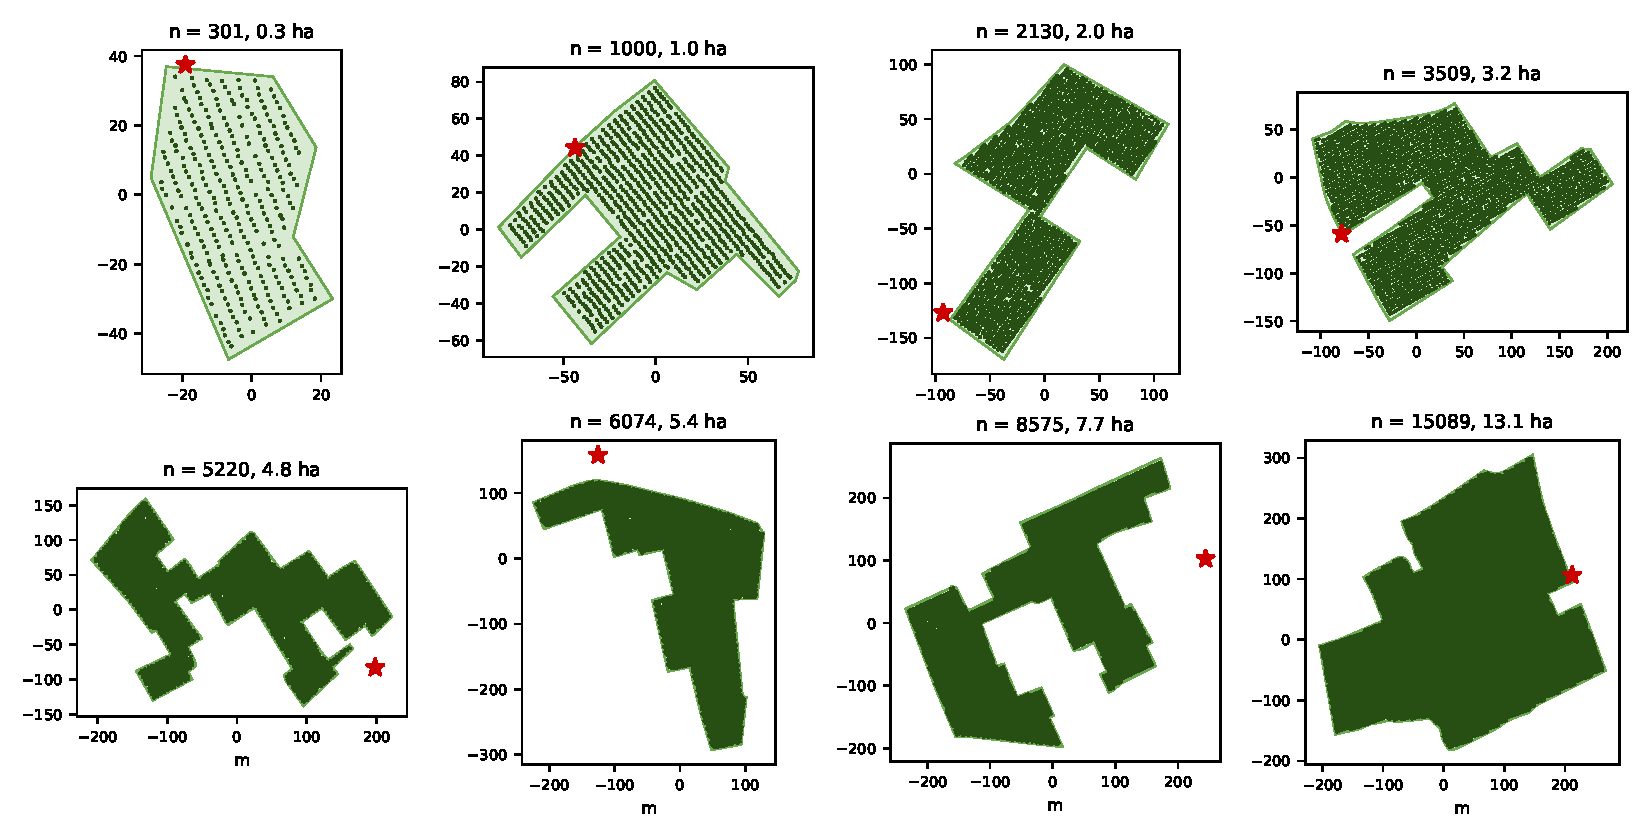
\includegraphics[width=\textwidth]{figs/fig_osm.pdf}
\caption{On altı gerçek bahçe sınırından sekizi (OpenStreetMap,
Isparta), üretilen ağaç kafesi ve depo (yıldız) ile birlikte}\label{fig:osm}
\end{figure}

\subsection{Yöntemler}
\begin{description}
\item[PSB+LNS (bu çalışma).] Algoritma~\ref{alg:psb}; tek atış PSB sonucu ve her
LNS iyileşmesi zaman damgasıyla kaydedilmiştir.
\item[LKH-3.] Sürüm 3.0.13, \texttt{MTSP\_OBJECTIVE = MINMAX}, \texttt{RUNS = 1};
üç yapılandırmada çalıştırılmıştır: \emph{varsayılan}; \emph{ayarlı}, yani iki bahçe
($n=467$ ve $1885$, $k=8$, 120\,s) üzerinde yapılan bir ön denemede sınanan altı ayardan en iyisi olan
\texttt{INITIAL\_TOUR\_}\allowbreak\texttt{ALGORITHM = MTSP} ve
\texttt{MOVE\_TYPE = 2} ($n=1885$ için bu ayar 120\,s'de \num{61249} değerine ulaşmış, varsayılan
ayar ise 600\,s sonunda \num{107222} değerinde kalmıştır); ve \emph{sıcak başlangıçlı}, yani tek atış
PSB çözümünden başlatılan ayarlı yapılandırma (\texttt{INITIAL\_TOUR\_}\allowbreak\texttt{FILE}; PSB
süresi bu yapılandırmanın ölçülen süresine dâhil edilmiştir).
\item[Literatürde öne çıkan min--maks mTSP kodları.] Kodu herkese açık olan dört yöntem
çalıştırılmıştır: HSNR \citep{hehao2022} (C++ kaynak kodu, \texttt{-O3} ile derlenmiş),
MA \citep{hehao2023} ve MILS \citep{hehaoxia2024} (yazarlarca dağıtılan Linux yürütülebilir
dosyaları) ve HGA \citep{mahmoudinazlou2024} (Julia kaynak kodu, tek iş parçacığı);
her biri varsayılan parametreleriyle, tek koşu hâlinde, bütçeye eşit bir duvar saati süre sınırıyla
ve koşuyu erken sonlandıramayan bir durdurma ölçütüyle çalıştırılmıştır. ITSHA \citep{zheng2022} ve
pekiştirmeli öğrenme tabanlı CMSA \citep{rodriguez2026} için açık kod bulunmamaktadır. MA
ve MILS yürütülebilir dosyaları, örnek başlığındaki şehir sayısını depo dâhil olarak
yorumlamaktadır; bu dosyalarla birlikte dağıtılan örnek dosyaları ise sayıyı depo hariç vermekte ve bu durum
son müşterinin uyarı verilmeden atlanmasına yol açmaktadır; bu nedenle başlık $n+1$ ile yazılmış ve her müşterinin
döndürülen rotalarda tam olarak bir kez yer aldığı doğrulanmıştır. MA yaklaşık $1.6\times10^{-7}n^2$\,GB
bellek gerektirdiğinden 15\,089 ağaçlı bahçede çalıştırılmamıştır (tahmini 36\,GB).
\end{description}

\subsection{Protokol ve ölçütler}
Her koşuda tek çekirdek kullanılmıştır. Deneyler, 12 çekirdekli/24 iş parçacıklı bir AMD Ryzen~9 3900X
işlemci ve 46\,GB bellek bulunan bir makinede yürütülmüştür; yöntemler iç içe sıralanarak 20 koşu eşzamanlı
çalıştırılmış, böylece makine yükünün tüm yöntemleri eşit biçimde etkilemesi sağlanmıştır. Zaman bütçesi
$n<1000$ için 120\,s, $n<5000$ için 300\,s, diğer durumlarda 600\,s olarak belirlenmiştir. PSB+LNS ve LKH-3
\SeedsMain{} tohumla (LNS ve LKH-3 için rastgele tohum; tek atış PSB sonucu
deterministiktir), literatürde öne çıkan dört kod ise tek tohumla çalıştırılmıştır. İyileşme izleri,
çıktı satırları üretildikçe duvar saatine göre zaman damgasıyla kaydedilmiştir; bir $b$ bütçesi,
$1.02\,b$ anına kadar ($b\ge 60$\,s için artı 2\,s) bir çözüm raporlanmışsa karşılanmış
sayılmış ve her yöntemin nihai sonucu, ilgili sınıf bütçesinin bu tolerans içinde kalan en iyi
çözümü olarak alınmıştır.

Her örnek ve $k$ değeri için \emph{best} (en iyi), herhangi bir yöntem, tohum ve süreyle bulunan en küçük
tamamlanma süresidir. Raporlanan ölçüler şunlardır: $t\in\{0.1,1,10,60\}$\,s bütçelerinde
ve bütçe sonunda $C_{\max}(t)/\text{best}-1$ sapması (çözüm yoksa ``çözüm yok''),
PSB+LNS'nin bir rakipten kesin olarak daha iyi olduğu örneklerin payı
(tohum ortalamaları kullanılarak) ve örnek başına ortalama nihai sapmalara
örnekler genelinde uygulanan çift yönlü Wilcoxon işaretli sıra testidir. Aynı temel
nokta kümesinin farklı $k$ değerleri bağımsız örnekler olmadığından $p$-değerleri
doğrulayıcı değil, keşifsel karşılaştırma ölçütleri olarak yorumlanmıştır.

\section{Kıyaslama sonuçları}\label{sec:results}

\subsection{Zamana göre çözüm kalitesi}
Şekil~\ref{fig:anytime}, sekiz yöntemin tamamı için bulunan en iyi tamamlanma süresine göre
medyan sapmayı duvar saati süresinin fonksiyonu olarak göstermektedir (ikinci panelde,
birinci panelde gösterilen mTSPLib örnekleri hariç tutulmuştur). Tablo~\ref{tab:sota} ise
örnek boyutuna göre ilk çözüme kadar geçen süreyi ve sabit bütçelerdeki sapmaları, bütçe
sonunda PSB+LNS'nin daha iyi olduğu örneklerin payı ve Wilcoxon $p$-değeri ile birlikte
listelemektedir. Tablo~\ref{tab:budget}, üç LKH-3
yapılandırması için karşılık gelen değerleri vermektedir. Sonuçlarda üç farklı rejim belirmiştir.

\begin{figure}[t]
\centering
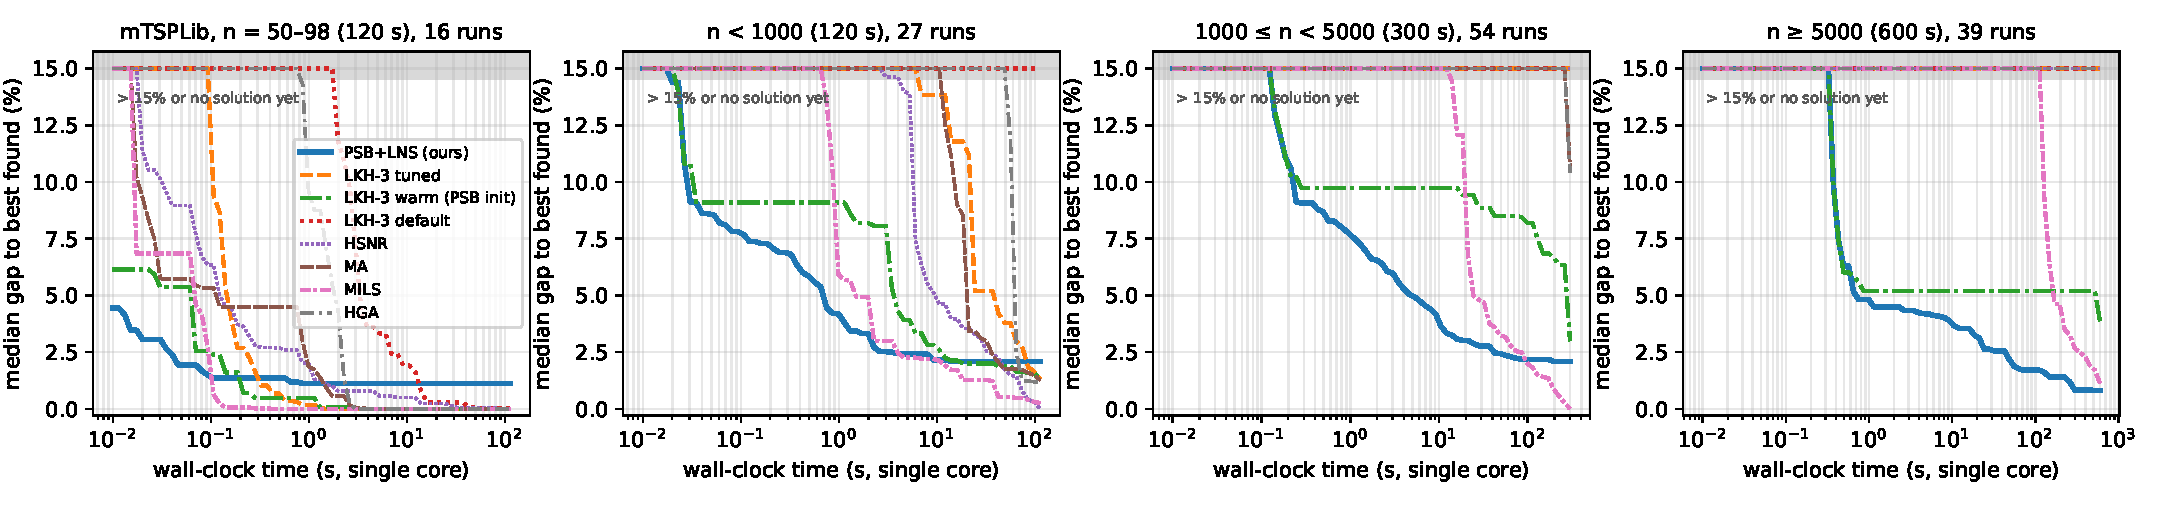
\includegraphics[width=\textwidth]{figs/fig_anytime.pdf}
\caption{Bulunan en iyi tamamlanma süresine göre medyan sapmanın duvar saati süresiyle
değişimi (tek çekirdek, logaritmik ölçek). Gölgeli bant: 15\% üzerinde sapma ya da henüz çözüm yok}\label{fig:anytime}
\end{figure}

\begin{table}[t]
\centering
\caption{Örnek boyutuna göre PSB+LNS ile literatürde öne çıkan kodların ve ayarlı LKH-3'ün
karşılaştırılması: ilk çözüme kadar geçen medyan süre ve bulunan en iyi tamamlanma süresine
göre medyan sapma (\%) ($\infty$: henüz çözüm yok). İlk çözüm medyanı yalnızca çözüm
döndüren koşuları, Wilcoxon testi iki yöntemin de sonlu nihai sonucu bulunan örnekleri
kapsar; büyük örneklerde HGA için test örneklem sayısı \SotaHgaWilcoxNLarge{}}\label{tab:sota}
\footnotesize
\setlength{\tabcolsep}{4pt}
\begin{tabular}{lrrrrrrr}
\toprule
method & first sol.\ [s] & 1\,s & 10\,s & 60\,s & final & PSB better [\%] & $p$ \\
\midrule
\multicolumn{8}{l}{\emph{$n<1000$, 43 instances}} \\
PSB+LNS (ours) & 0.01 & 2.43 & 1.77 & 1.63 & 1.63 & -- & -- \\
MILS & 0.08 & 3.58 & 1.12 & 0.01 & 0.00 & 23 & 3e-04 \\
HGA & 3.11 & \ensuremath{\infty} & 14.37 & 0.87 & 0.48 & 26 & 1e-02 \\
MA & 0.10 & 6.78 & 3.23 & 0.54 & 0.35 & 21 & 5e-03 \\
HSNR & 0.08 & 7.93 & 1.31 & 0.26 & 0.00 & 19 & 7e-03 \\
LKH-3 tuned & 2.04 & \ensuremath{\infty} & 2.10 & 0.86 & 0.57 & 28 & 6e-01 \\
\midrule
\multicolumn{8}{l}{\emph{$1000\le n<5000$, 54 instances}} \\
PSB+LNS (ours) & 0.10 & 7.70 & 3.82 & 2.29 & 2.08 & -- & -- \\
MILS & 4.73 & \ensuremath{\infty} & 23.04 & 2.90 & 0.00 & 17 & 4e-07 \\
HGA & 52.57 & \ensuremath{\infty} & \ensuremath{\infty} & \ensuremath{\infty} & 10.42 & 91 & 7e-10 \\
MA & 8.83 & \ensuremath{\infty} & 36.62 & 23.95 & 10.31 & 89 & 3e-09 \\
HSNR & 30.33 & \ensuremath{\infty} & \ensuremath{\infty} & 41.19 & 15.05 & 83 & 5e-09 \\
LKH-3 tuned & 244.97 & \ensuremath{\infty} & \ensuremath{\infty} & \ensuremath{\infty} & 31.53 & 85 & 2e-09 \\
\midrule
\multicolumn{8}{l}{\emph{$n\ge 5000$, 39 instances}} \\
PSB+LNS (ours) & 0.33 & 4.82 & 3.65 & 1.82 & 0.81 & -- & -- \\
MILS & 46.48 & \ensuremath{\infty} & \ensuremath{\infty} & 60.46 & 1.13 & 54 & 5e-01 \\
HGA & 1007.72 & \ensuremath{\infty} & \ensuremath{\infty} & \ensuremath{\infty} & \ensuremath{\infty} & 100 & 6e-02 \\
MA & 124.73 & \ensuremath{\infty} & \ensuremath{\infty} & \ensuremath{\infty} & 27.17 & 100 & 2e-10 \\
HSNR & 606.54 & \ensuremath{\infty} & \ensuremath{\infty} & \ensuremath{\infty} & 59.92 & 100 & 2e-06 \\
LKH-3 tuned & 600.87 & \ensuremath{\infty} & \ensuremath{\infty} & \ensuremath{\infty} & 97.14 & 100 & 4e-12 \\
\bottomrule
\end{tabular}

\end{table}

\paragraph{Küçük örnekler ($n<1000$)} Birkaç saniyeden fazla süre bulunduğunda bu
grupta klasik çözücüler tercih edilmelidir. MILS 60\,s sonunda 0.01\% medyan sapmaya
ulaşmış, PSB+LNS ise \CountSmall{} örneğin yalnızca \SotaMilsWinSmall\% kadarında MILS'ten
daha iyi sonuç vermiştir; ayarlı LKH-3 karşısındaki fark anlamlı bulunmamıştır
($p=\PvsTunedSmall$). PSB+LNS yalnızca ilk saniyelerde önde kalmıştır.

\paragraph{Orta büyüklükteki örnekler ($1000\le n<5000$)} PSB ilk çözümünü medyan 0.1\,s sonra,
MILS \SotaMilsFirstMid\,s sonra, MA, HSNR ve HGA 9 ile
53\,s arasında, ayarlı LKH-3 ise yaklaşık dört dakika sonra döndürmüştür. 10\,s anında
PSB+LNS, \CountMid{} örneğin \SotaMilsWinTenMid\% kadarında MILS'ten daha iyi sonuç vermiştir (MILS'in medyan sapması:
\SotaMilsTenMid\%). MILS yaklaşık iki dakika sonra PSB+LNS'yi geçmiş ve 300\,s'lik bütçenin
sonunda örneklerin çoğunda daha iyi sonuç vermiştir (PSB+LNS'nin daha iyi olduğu pay:
\SotaMilsWinMid\%). PSB+LNS, bütçe sonunda örneklerin 83--91\% kadarında HGA, MA, HSNR ve
ayarlı LKH-3'ten daha iyi sonuç vermiştir (tümünde $p<10^{-8}$).

\paragraph{Büyük örnekler ($n\ge 5000$)} 600\,s'lik bütçenin tamamı boyunca en düşük
medyan sapmayı PSB+LNS vermiştir. MILS ilk çözümünü medyan
\SotaMilsFirstLarge\,s sonra bildirmiş ve bütçe sonunda PSB+LNS ile başa baş kalmıştır
(\CountLarge{} örneğin \SotaMilsWinLarge\% kadarında PSB+LNS daha iyi, $p=\SotaMilsPLarge$); MA,
HSNR ve HGA çok geride kalmış, ayarlı LKH-3 ise hiçbir örnekte 60\,s içinde çözüm
bildirmemiş ve bütçeyi \TunedFinalLarge\% medyan sapmayla tamamlamıştır.

\InstAll{} örneğin tamamı üzerinde PSB+LNS, 1\,s sonunda örneklerin \SotaMilsWinOneAll\%
kadarında, 10\,s sonunda \SotaMilsWinTenAll\% kadarında ve bütçe sonunda \SotaMilsWinAll\%
kadarında MILS'ten daha iyi sonuç vermiştir; HGA, MA ve HSNR karşısındaki nihai paylar sırasıyla
\SotaHgaWinAll\%, \SotaMaWinAll\% ve \SotaHsnrWinAll\%, ayarlı LKH-3 karşısında ise
\WinFinalAll\% olmuştur ($p=\PvsTunedAll$). Nihai PSB+LNS sapma değerlerinin \SeedsMain{} tohum
arasındaki standart sapmasının medyanı \PsbSeedSdAll{} yüzde puan olmuştur.

\begin{table}[t]
\centering
\caption{PSB+LNS ve LKH-3: sabit bütçelerde, bulunan en iyi tamamlanma süresine göre medyan
sapma (\%) ($\infty$: henüz çözüm yok; çözüm bulunamayan koşuların payı
parantez içinde)}\label{tab:budget}
\footnotesize
\setlength{\tabcolsep}{4pt}
\begin{tabular}{lrrrrrr}
\toprule
method & 0.1\,s & 1\,s & 10\,s & 60\,s & cap & final \\
\midrule
\multicolumn{7}{l}{\emph{mTSPLib, 16 instances, cap 120\,s}} \\
PSB+LNS & 1.36 & 1.13 & 1.13 & 1.13 & -- & 1.13 \\
LKH-3 tuned & 9.39\,{\scriptsize(40\%)} & 0.17 & 0.00 & 0.00 & -- & \textbf{0.00} \\
LKH-3 warm & 2.54 & 0.47 & 0.00 & 0.00 & -- & 0.00 \\
LKH-3 default & \ensuremath{\infty}\,{\scriptsize(100\%)} & \ensuremath{\infty}\,{\scriptsize(69\%)} & 1.91 & 0.05 & -- & 0.01 \\
\midrule
\multicolumn{7}{l}{\emph{$n<1000$, 43 instances, cap 120\,s}} \\
PSB+LNS & 5.93 & 2.43 & 1.77 & 1.63 & -- & 1.63 \\
LKH-3 tuned & \ensuremath{\infty}\,{\scriptsize(78\%)} & \ensuremath{\infty}\,{\scriptsize(61\%)} & 2.10\,{\scriptsize(16\%)} & 0.86\,{\scriptsize(1\%)} & -- & 0.57 \\
LKH-3 warm & 8.16 & 6.51 & 1.78 & 0.44 & -- & \textbf{0.43} \\
LKH-3 default & \ensuremath{\infty}\,{\scriptsize(100\%)} & \ensuremath{\infty}\,{\scriptsize(88\%)} & \ensuremath{\infty}\,{\scriptsize(63\%)} & 30.48\,{\scriptsize(44\%)} & -- & 3.15 \\
\midrule
\multicolumn{7}{l}{\emph{$1000\le n<5000$, 54 instances, cap 300\,s}} \\
PSB+LNS & \ensuremath{\infty}\,{\scriptsize(48\%)} & 7.70 & 3.82 & 2.29 & 2.08 & \textbf{2.08} \\
LKH-3 tuned & \ensuremath{\infty}\,{\scriptsize(100\%)} & \ensuremath{\infty}\,{\scriptsize(100\%)} & \ensuremath{\infty}\,{\scriptsize(100\%)} & \ensuremath{\infty}\,{\scriptsize(84\%)} & 31.53 & 31.53 \\
LKH-3 warm & \ensuremath{\infty}\,{\scriptsize(52\%)} & 9.72 & 9.72 & 8.50 & 2.99 & 2.99 \\
LKH-3 default & \ensuremath{\infty}\,{\scriptsize(100\%)} & \ensuremath{\infty}\,{\scriptsize(100\%)} & \ensuremath{\infty}\,{\scriptsize(100\%)} & \ensuremath{\infty}\,{\scriptsize(100\%)} & 242.83\,{\scriptsize(30\%)} & 242.83 \\
\midrule
\multicolumn{7}{l}{\emph{$n\ge 5000$, 39 instances, cap 600\,s}} \\
PSB+LNS & \ensuremath{\infty}\,{\scriptsize(100\%)} & 4.82\,{\scriptsize(1\%)} & 3.65 & 1.82 & 0.81 & \textbf{0.81} \\
LKH-3 tuned & \ensuremath{\infty}\,{\scriptsize(100\%)} & \ensuremath{\infty}\,{\scriptsize(100\%)} & \ensuremath{\infty}\,{\scriptsize(100\%)} & \ensuremath{\infty}\,{\scriptsize(100\%)} & 97.14 & 97.14 \\
LKH-3 warm & \ensuremath{\infty}\,{\scriptsize(100\%)} & 5.20 & 5.20 & 5.20 & 3.87 & 3.87 \\
LKH-3 default & \ensuremath{\infty}\,{\scriptsize(100\%)} & \ensuremath{\infty}\,{\scriptsize(100\%)} & \ensuremath{\infty}\,{\scriptsize(100\%)} & \ensuremath{\infty}\,{\scriptsize(100\%)} & \ensuremath{\infty}\,{\scriptsize(85\%)} & \ensuremath{\infty} \\
\bottomrule
\end{tabular}

\end{table}

LKH-3'ün PSB çözümünden sıcak başlangıçla çalıştırılması, ilk tur için gereken uzun bekleme süresini ortadan
kaldırmıştır; ancak Şekil~\ref{fig:anytime} üzerindeki eğrilerinde görülen düz kesimler, bütçenin
büyük kısmının başlangıç çözümü iyileştirilmeden geçtiğini göstermektedir. Bütçe
sonunda PSB+LNS, orta büyüklükteki örneklerin \WinWarmMid\% kadarında ve büyük örneklerin
\WinWarmLarge\% kadarında sıcak başlangıçlı LKH-3'ten daha iyi sonuç vermiştir.

\subsection{Kurulum süresi, ölçeklenme ve paralellik}
LNS olmadan PSB, medyan \PsbOneShotMs\,ms sonra, bulunan en iyi tamamlanma süresine göre
medyan sapması \PsbOneShotGap\% olan bir çözüm döndürmüştür; ayarlı LKH-3 ise örneklerin
\ReachNeverAll\% kadarında bütçesi içinde bu kaliteye ulaşamamıştır. Tek atış
süresi $n$ ile neredeyse doğrusal olarak artmıştır (uydurulan üs \ScaleExponent;
$n=\ScaleNLargest$ için \ScaleMsLargest\,ms). Rota başına hesaplama çekirdeklerinin dört
veya daha fazla iş parçacığında çalıştırılması kurulumu hızlandırmamış, aksine yavaşlatmıştır
(medyan hızlanma \ScaleSpeedupFour); bunun nedeni, dev tur ve bölme adımlarının hesaplama süresine
hâkim olması ve sıralı yürütülmesidir. Bu nedenle tüm sonuçlarda tek çekirdek kullanılmıştır.

\subsection{Ablasyon}
Tablo~\ref{tab:ablation}, her seferinde bir bileşen çıkarılarak ya da değiştirilerek elde
edilen medyan tek atış tamamlanma süresini tam işlem hattına göre vermektedir. Dengeleme
yaklaşık 2\% (tüm örnekler üzerinde \AblNoBalanceAll\%), optimal bölme eşit uzunluklu
bölmeye karşı \AblEqualSplitAll\%, dev tur üzerindeki yerel arama ise yaklaşık 1.5\%
katkı sağlamıştır. Önce küme, sonra rota yaklaşımına dayalı alternatifler belirgin biçimde daha kötü sonuç vermiştir:
her küme için ayrı bir TSP çözülen $k$-means yaklaşımı \AblKmeansTspAll\%, PSB dengeleme adımı eklendiğinde
bile \AblKmeansBalAll\% kayba yol açmıştır. Depo çevresinde açısal tarama, düzenli
sentetik bahçelerde PSB'ye çok yakın bir medyan vermiş (\AblSweepTspOrchard\%), ancak gerçek
bahçe sınırlarında \AblSweepTspOsm\%, VLSI örneklerinde ise \AblSweepTspVlsi\% kayba yol açmıştır;
30\,s'lik LNS sonrasında başlangıç seçiminin etkisi küçük kalmıştır (tarama
başlangıcı için \LnsStartOrchard\% ve \LnsStartVlsi\%). Bu bulgu, kurulum adımının asıl katkısının
erken aşamada iyi bir çözüm sağlamak olduğunu göstermektedir.

\begin{table}[t]
\centering
\caption{Tek atış kurulum adımının ablasyonu: tam PSB işlem hattına göre medyan tamamlanma süresi
(\%) ve medyan süre; sent.: sentetik bahçeler, gerçek: gerçek
bahçe sınırları, lit.: literatür kümesi (örnek sayıları parantez içinde)}\label{tab:ablation}
\scriptsize
\setlength{\tabcolsep}{2.5pt}
\begin{tabular}{lrrrrrr}
\toprule
variant & mTSPLib (16) & synth. (48) & real (48) & VLSI (24) & lit. (52) & time [ms] \\
\midrule
PSB (full) & -- & -- & -- & -- & -- & 80 \\
no Balance & +2.70 & +1.82 & +2.31 & +1.68 & +2.58 & 44 \\
no Polish, no Balance & +4.25 & +2.28 & +2.43 & +1.84 & +2.76 & 26 \\
equal-length split & +0.00 & +1.06 & +1.34 & +5.54 & +4.12 & 106 \\
GE tour, no 2-opt/Or-opt & +1.20 & +1.35 & -0.17 & +1.67 & +1.62 & 87 \\
nearest-neighbour tour & +0.25 & +0.75 & +0.63 & +1.11 & +0.13 & 186 \\
sweep + TSP & +1.55 & +0.09 & +6.37 & +6.30 & +3.68 & 33 \\
$k$-means + TSP & +13.03 & +26.03 & +26.44 & +20.49 & +20.56 & 35 \\
$k$-means + TSP + Balance & +2.70 & +11.67 & +13.61 & +7.48 & +5.78 & 101 \\
\bottomrule
\end{tabular}

\end{table}

\subsection{Literatür kıyaslaması}
Ek~A, $\mathbb{S}$ ve $\mathbb{L}$ kümelerindeki
\LitCount{} örneğin referans değerlerine göre sapmalarını listelemektedir. Referans değerler
birkaç saate kadar süren koşulardan elde edilmiştir \citep{hehaoxia2024}; burada ise en
fazla 600\,s süren tek bir koşu yapılmıştır. PSB+LNS hiçbir referans değeri iyileştirmemiştir.
Az sayıda robotun kullanıldığı örneklerde ($k\le 5$, \LitFewKCount{} örnek) PSB+LNS'nin medyan sapması
\LitFewKPsbFinal\% olmuş, bu değer MILS için \LitFewKMilsFinal\%, ayarlı LKH-3 için
\LitFewKTunedFinal\% olarak bulunmuştur; çok sayıda robotun kullanıldığı örneklerde ($k\ge 10$) ise medyanlar sırasıyla
\LitManyKPsbFinal\%, \LitManyKMilsFinal\% ve \LitManyKTunedFinal\% olmuştur. Her iki grupta
da bütçe sonunda en düşük sapmayı MILS sağlamış, PSB+LNS ise çok sayıda robot içeren
\LitManyKCount{} örneğin \LitManyKPsbBeatsTuned{} tanesinde ayarlı LKH-3'ten daha iyi
sonuç vermiştir.

\subsection{Mutlak kalite}
Nihai PSB+LNS tamamlanma süresinin alt sınır~\eqref{eq:lb} değerine göre medyan sapması
sentetik bahçelerde \LbGapOrch\%, VLSI örneklerinde \LbGapVlsi\% ve mTSPLib örneklerinde
\LbGapMtsp\% olmuştur; bu farkın bir kısmı, ne en uzak hedef teriminin ne de MST teriminin baskın
olduğu durumlarda sınırın zayıf kalmasından kaynaklanmaktadır.

\section{Kablolu drone platformlarıyla seçmeli elma hasadı}\label{sec:harvest}

Kıyaslamada tamamlanma süresi sabit bir bütçede ölçülmüştür. Bir hasat operasyonunda ise plan,
bir platform kasa değişimi için her döndüğünde yeniden hesaplanır, ağaç başına meyve
sayıları ağaçlar gözlemlenene kadar belirsiz kalır ve hareket sıra aralarıyla
sınırlıdır. Bu bölümde planlayıcılar, böyle bir operasyonun ayrık olaylı benzetiminde
değerlendirilmiştir; benzetim parametreleri, değer bulunabilen her durumda
tarım literatüründen alınmıştır.

\subsection{Senaryo}

\begin{figure}[t]
\centering
\begin{minipage}{0.485\textwidth}\centering
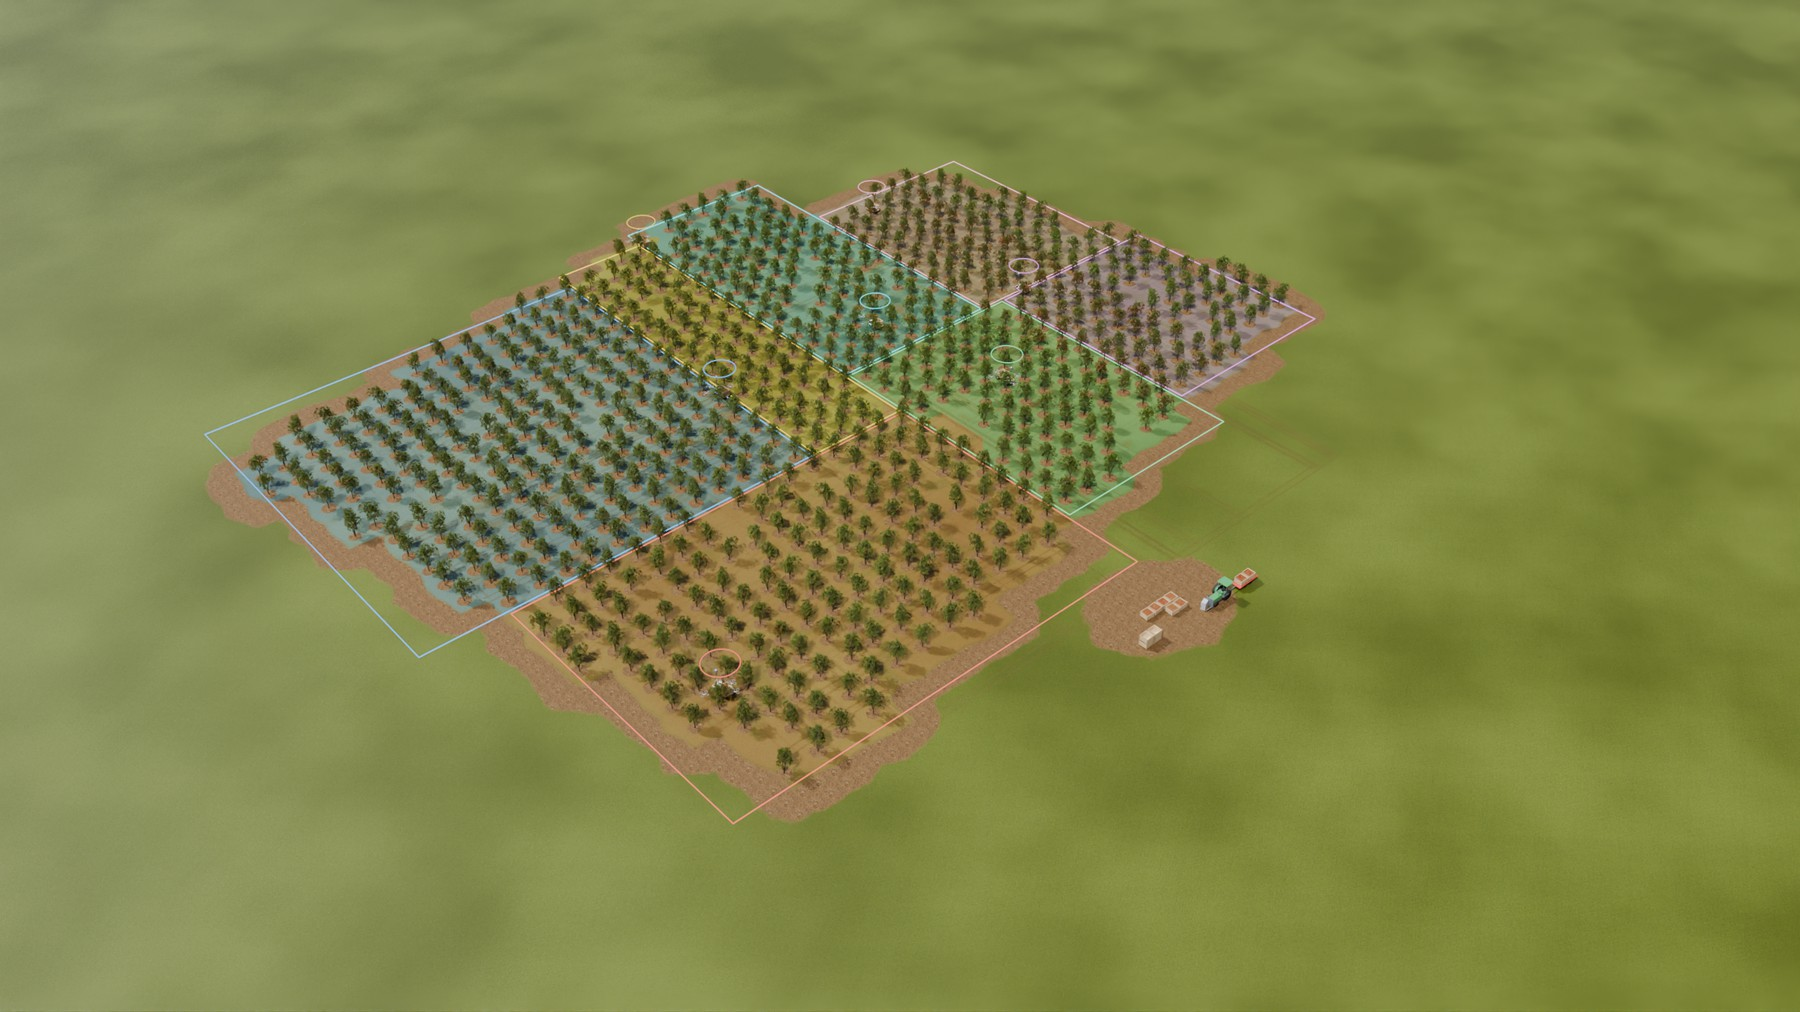
\includegraphics[width=\linewidth]{figs/fig_v4_overview.jpg}\\(a)
\end{minipage}\hfill
\begin{minipage}{0.485\textwidth}\centering
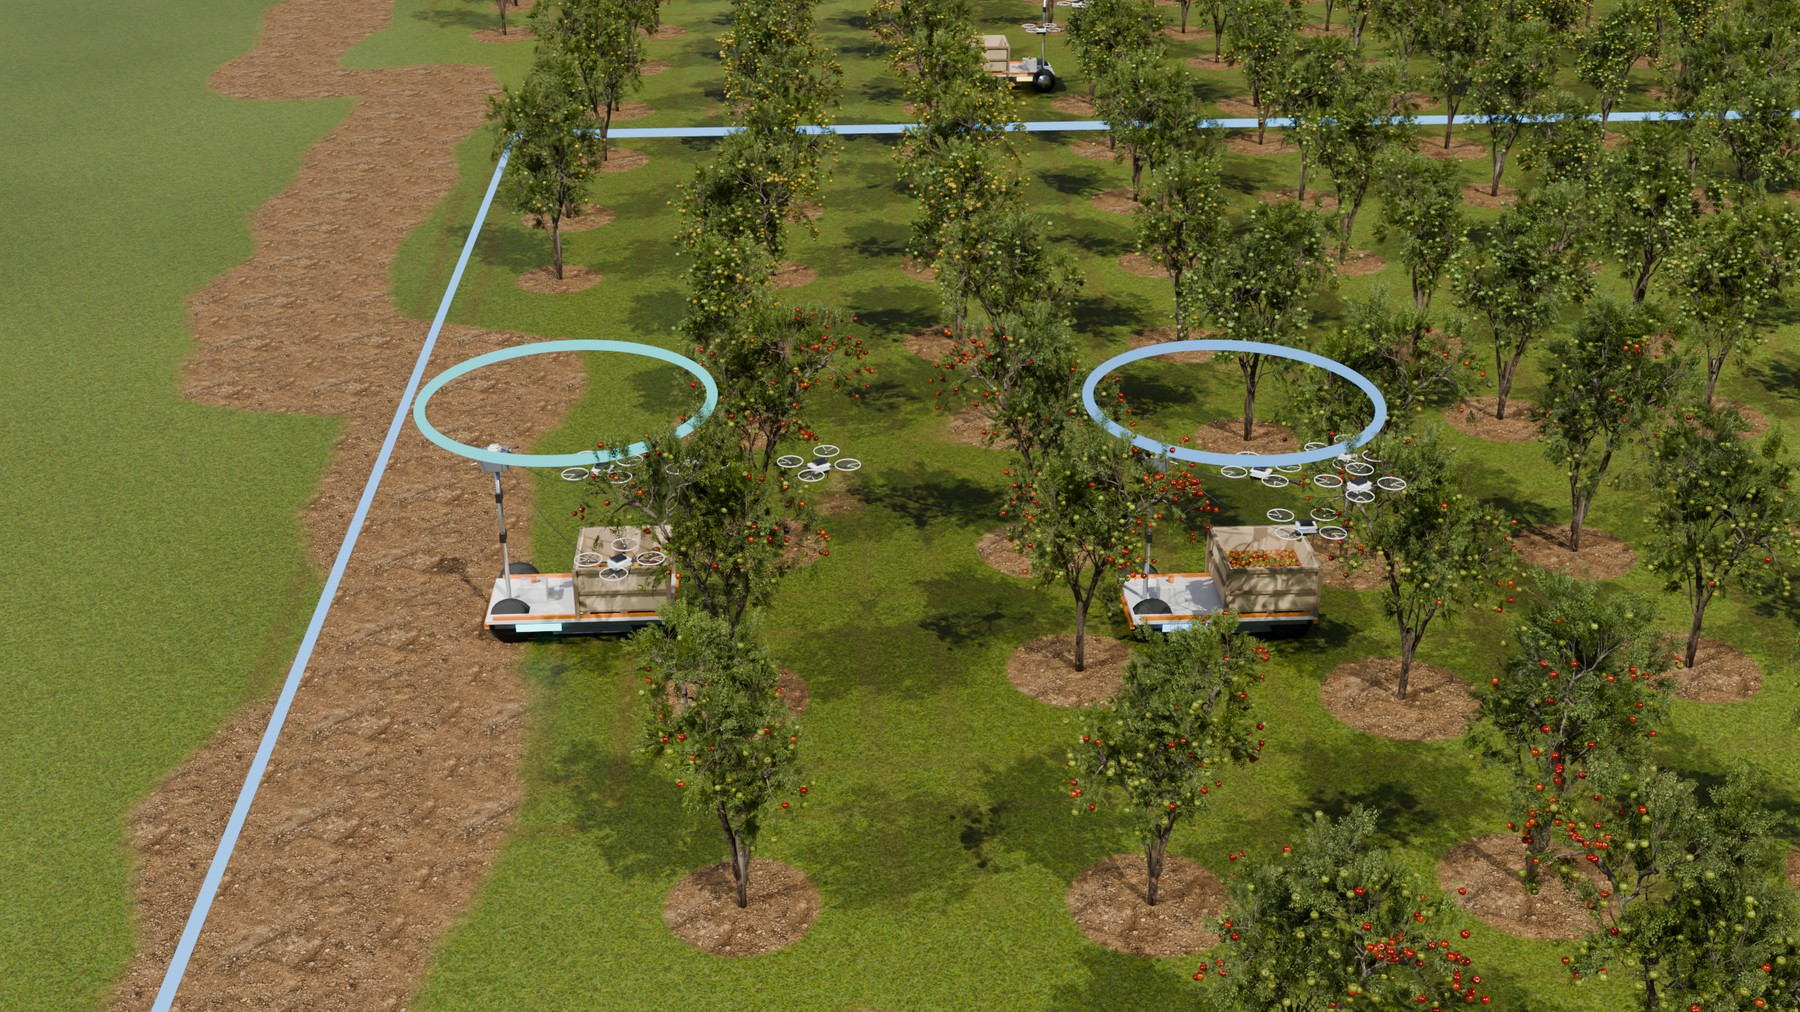
\includegraphics[width=\linewidth]{figs/fig_v4_takeover.jpg}\\(b)
\end{minipage}\\[4pt]
\begin{minipage}{0.485\textwidth}\centering
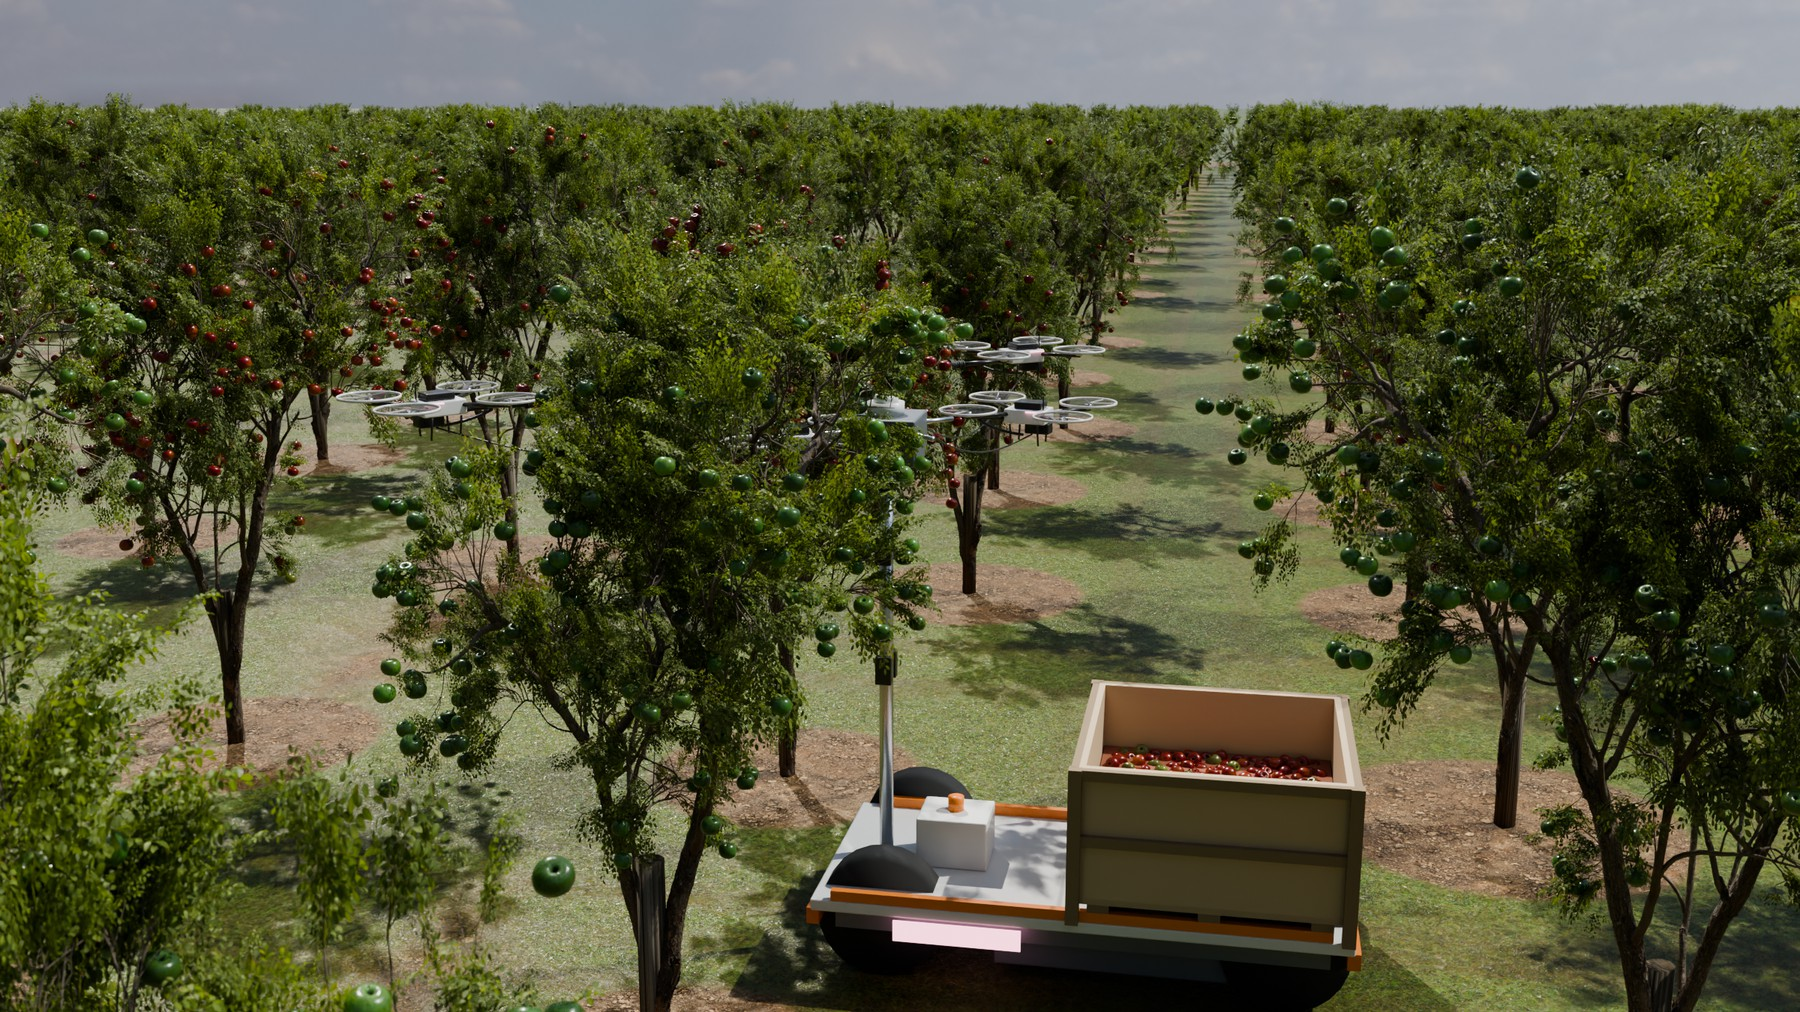
\includegraphics[width=\linewidth]{figs/fig_v4_platform.jpg}\\(c)
\end{minipage}\hfill
\begin{minipage}{0.485\textwidth}\centering
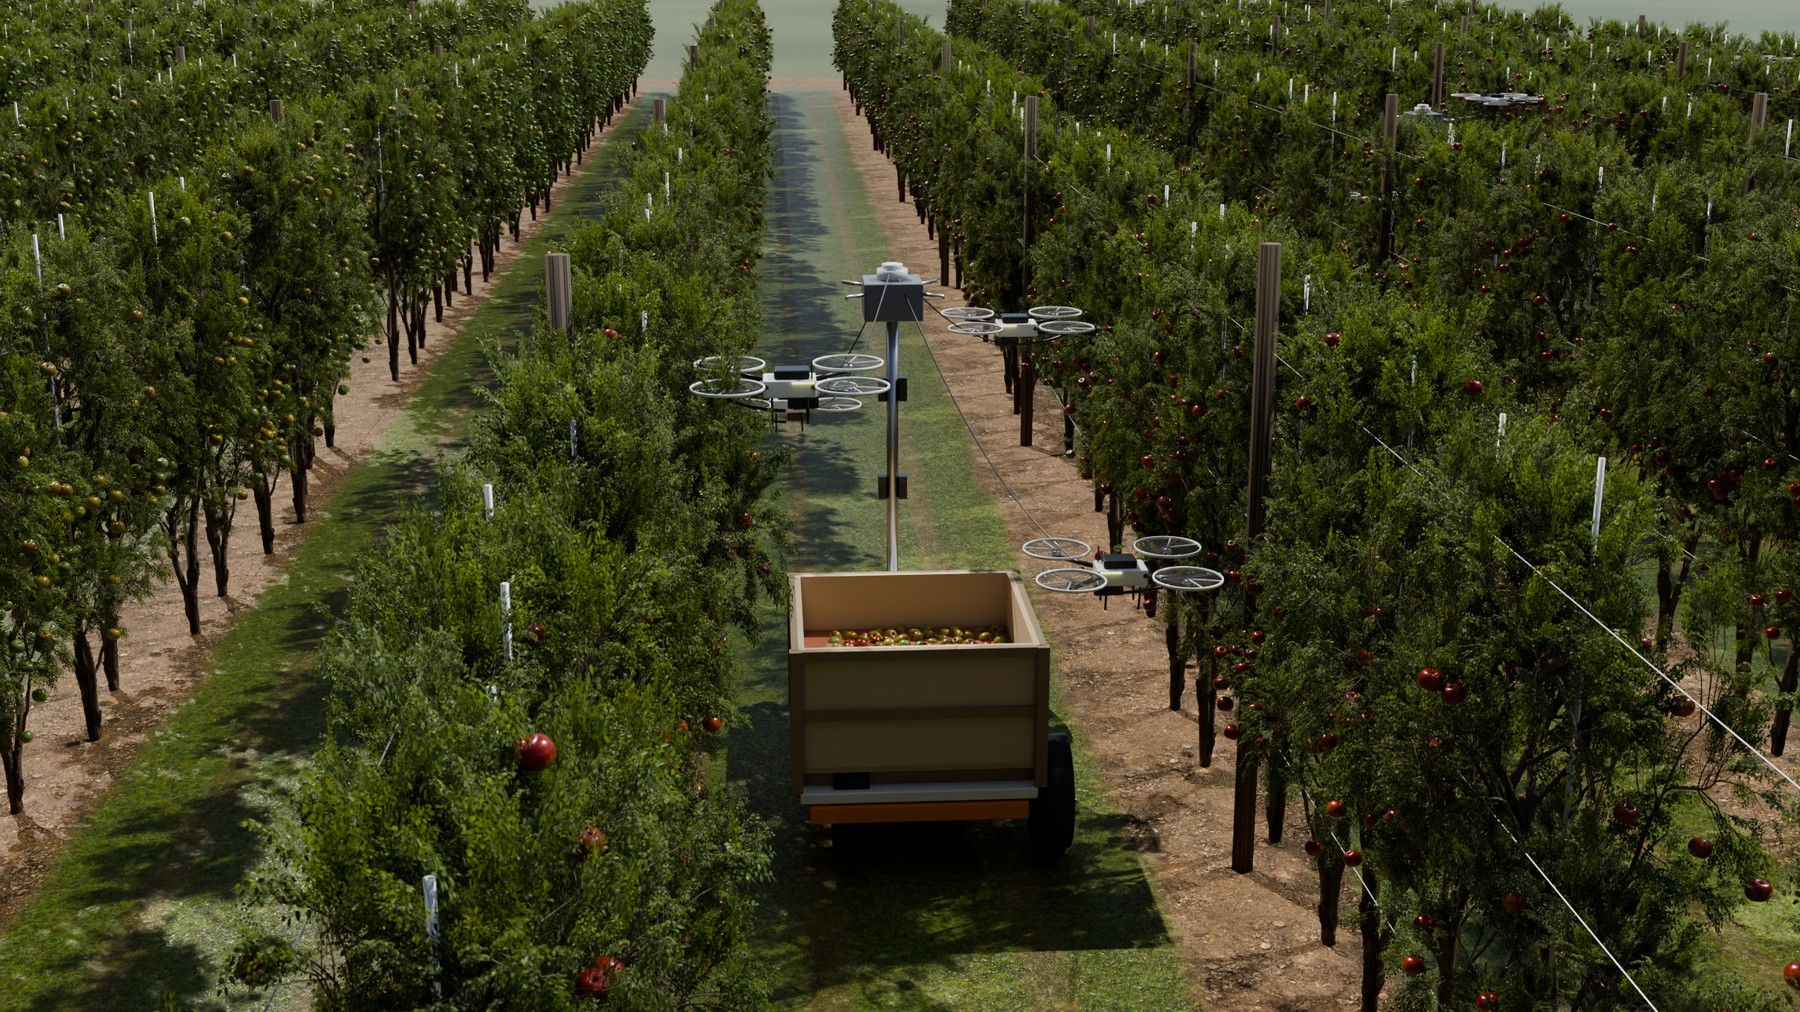
\includegraphics[width=\linewidth]{figs/fig_v3_platform.jpg}\\(d)
\end{minipage}
\caption{Benzetimi yapılan görevlerin yeniden oynatımı: (a) $k$-d bölgeleriyle kare dikimli
bahçe; (b) uç devralma; (c) bir sıra arası kesişiminde dört kablolu drone taşıyan
platform; (d) Tall Spindle bahçesi}\label{fig:blender}
\end{figure}

Benzetimde, her biri bir kasa ile dört drone'un kabloyla bağlandığı bir merkez birimi taşıyan
yer platformlarından oluşan bir filo modellenmiştir (Şekil~\ref{fig:blender}); bu kurgu, sektör
basınında tanıtılan kablolu meyve toplama robotlarından esinlenmiştir \citep{oitzman_2021_tevel,coxworth_2022_fruitpicking}.
Bu tür sistemlere ilişkin hakemli performans verisi bulunmadığından, sistem parametreleri
duyarlılık analizinde değiştirilmiştir. Senaryo, taze tüketim pazarına yönelik seçmeli
bir toplamadır: yalnızca olgun meyveler toplanır ve kasaya yerleştirilir. Taze tüketime
yönelik elmalar küçük düşme yüksekliklerinde bile ezildiğinden \citep{schulte_1992_apple}
ve yere temas ettikten sonra taze tüketim için satılamadığından \citep{ewing_2018_food},
meyvenin düşürülmesi bu elmalar için bir seçenek değildir; sanayilik elmalar ise sıra
üstü sarsıcılarla çok daha hızlı hasat edilmektedir \citep{brawner_2025_overtherow}; bu nedenle
seçmeli drone hasadı yalnızca taze tüketim pazarı için anlamlıdır.

\subsection{Model}

\begin{table}[t]
\centering
\caption{Benzetim parametreleri. ``Varsayım'' ifadesi, ölçülmüş karşılığı bulunamayan
değerleri belirtir; duyarlılık analizi, aralık sütununda değer verilen parametrelerle
ve her seferinde tek parametre değiştirilerek sınırlandırılmıştır}\label{tab:params}
\scriptsize
\begin{tabular}{p{3.3cm}p{2.4cm}p{1.8cm}p{3.4cm}}
\toprule
parametre & değer & duyarlılık aralığı & kaynak \\
\midrule
\multicolumn{4}{l}{\emph{Bahçe}} \\
kare dikim aralığı & 4.0\,m $\times$ 4.0\,m ($\pm$5--10\%) & 3.5--5.0\,m & düşük yoğunluklu serbest duran sistemler \citealp{brawner_2026_wsu,robinson_2008_evolution} \\
Tall Spindle (sıralı bahçe durumu) & 0.9\,m $\times$ 3.3\,m & -- & \citealp{robinson_2011_tallspindle,hoying_nd_tallspindle,reig_2020_longterm} \\
konum gürültüsü, bükülmüş sıralar, boşluklar & 0.25\,m; 0.2--0.6\,m; 6\% + öbekler & 0.1--0.6\,m & varsayım \\
ağaç başına meyve (kare dikim; sıralı) & NB ortalaması 300; 130 & 150--450 & \citealp{francescatto_2020_precision} \\
meyve sayısı saçılımı / hedef eşiği & NB $r=5$ / 5 olgun meyve & -- & varsayım \\
çeşit, uzamsal alan ve meyve gürültüsü & üç kayma; 0.35; 0.35 & -- & varsayım \\
bir toplama geçişinde olgun meyve payı & 40\% (ilk), 15\% (seyrek) & -- & \citealp{simnitt_2023_advancements,hall_2001_effect}; varsayım \\
dış/üst meyvelerin daha erken olgunlaşması & evet & -- & \citealp{roper_2001_when,moran_2022_honeycrisp}; aksi yönde \citealp{kviklys_2022_apple} \\
\midrule
\multicolumn{4}{l}{\emph{Algılama ve toplama}} \\
ön kestirim hatası & log-normal, $\sigma=0.6$ & 0.3--0.9 & varsayım \\
geçiş sırasında görünür meyve payı & 0.60 & -- & \citealp{gongal_2016_apple} (vekil ölçüt) \\
tespit yakalama oranı / kesinlik & 0.85 / 0.88 & yakalama oranı 0.82--0.97 & \citealp{kang_2020_fast,sapkota_2024_comparing,genemola_2020_fruit} \\
girişim başına koparma başarısı & 0.80 & -- & \citealp{silwal_2017_design,zhang_2024_automated,zhu_2025_advancement} \\
toplama girişimi başına süre & 6.0\,s & 3.6--7.3\,s & \citealp{silwal_2017_design,zhang_2024_automated,hohimer_2019_design} \\
platform başına drone sayısı & 4 & 2--6 & \citealp{oitzman_2021_tevel,coxworth_2022_fruitpicking} (sektör basını) \\
\midrule
\multicolumn{4}{l}{\emph{Platform ve lojistik}} \\
sıra aralarında platform hızı & 1.0\,m/s & 0.5--2.0\,m/s & varsayım \\
durma / dönüş süresi & 20\,s / 20\,s & -- & varsayım \\
kasa kapasitesi & 2300 meyve ($\approx$380\,kg) & 1500--3000 & varsayım \\
istasyonda kasa değişim süresi & 120\,s & 60--300\,s & varsayım \\
\bottomrule
\end{tabular}

\end{table}

\paragraph{Bahçeler} Ana durum, platformların sıra aralarında her iki yönde de
ilerleyebildiği, serbest duran ağaçlardan oluşan kare dikimli bir bahçedir (yaklaşık
4\,m'ye 4\,m). Geometri bilinçli olarak kusurlu tutulmuş ve her tohumla değiştirilmiştir:
iki yöndeki aralıklar birbirinden 5--10\% farklıdır, sıralar 0.2--0.6\,m'lik düşük
frekanslı bir yer değiştirmeyle bükülmüş, her ağaç $\sigma=0.25$\,m standart sapmayla kaydırılmış,
ağaçların 6\%'sı rastgele çıkarılmış ve en fazla üç ölü ağaç öbeğiyle ek ağaçlar
kaldırılmıştır; sınır olarak ya çentikli 1.3\,ha'lık bir blok ya da Şekil~\ref{fig:osm}'deki
dört gerçek bahçe sınırından biri (1.0 ile 5.4\,ha arası) kullanılmış, bahçenin yönelimi ise planlayıcılara
bildirilmemiştir. Bahçelerde \HgTreesMin{} ile \HgTreesMax{} arasında ağaç
bulunmaktadır. Bu geometri, Isparta'nın en çok elma üreten ilçesi olan Gelendost'taki
\citep{sargin_2014_isparta} bahçelerin herkese açık uydu görüntüleriyle karşılaştırılmıştır
(ör. 38.125\,K, 31.025\,D). İncelediğimiz parsellerde hem kare dikimli (ağaç aralığı yaklaşık 5\,m)
hem de sıralı bahçeler yer almakta ve parsellerin çoğu 1\,ha'dan küçüktür. Benzetimdeki bahçeler
ise daha sık dikimli (4\,m) ve daha büyüktür; bükülmüş sıralar, eksik ağaçlar ve çentikli sınırlar
da bilinçli olarak belirgin tutulmuştur. Dolayısıyla benzetim, ağaç sayısı ve geometrik düzensizlik
bakımından bu bahçelerden daha zorlayıcıdır. İkinci durumda, dört sınır üzerinde yüksek yoğunluklu bir Tall Spindle
dikimi (0.9\,m'ye 3.3\,m) kullanılmıştır; bu durumda platformlar sıra aralarında kalmak zorundadır
ve bir sıra arasından diğerine baş tarla üzerinden geçer.

\paragraph{Meyve ve algılama} Kare dikimli ve sıralı bahçelerde ağaç başına
meyve sayısı sırasıyla $\mu=300$ ve $130$ olmak üzere
$N_i\sim\mathrm{NB}(5,5/(5+\mu))$ dağılımından üretilmiştir. Meyve $\ell$'nin
olgunluk puanı
$m_{i\ell}=b_{c(i)}+0.35z_i+0.45(U_{i\ell}-0.5)+\varepsilon_{i\ell}$,
$\varepsilon_{i\ell}\sim N(0,0.35^2)$ biçimindedir; $b_{c(i)}$ beş sıralık
bloklara atanan üç çeşidin kayması, $z_i$ on iki rastgele Gauss tepesinden oluşan,
standartlaştırılmış uzamsal alan ve $U_{i\ell}\sim U(0,1)$ dış/üst konum
avantajıdır. $m\ge0$ olan meyve olgun sayılmıştır. İlk geçişte çeşit kaymaları
$(0.148,-0.202,-0.602)$, seyrek geçişte $(-0.291,-0.641,-1.041)$ alınarak
hedef olgun payları yaklaşık \%40 ve \%15 olarak kalibre edilmiştir.

$R_i>0$ için ilk kestirim $R_i\exp(N(0,0.6^2))$, $R_i=0$ için Poisson(2)
değeridir. Kameralar 10\,m içindeki ağaçları gözler; gözlenen ağacın kestirimi,
$X_i\sim\mathrm{Binomial}(R_i,0.60)$ olmak üzere $X_i/0.60$ ile güncellenir.
Bu büyüklük doğrudan görünür meyve sayısı değil, görünürlük düzeltilmiş toplam
olgun meyve kestirimidir. Ziyaret edilen ağaçta tespit sayısı
$D_i\sim\mathrm{Binomial}(R_i,0.85)$ olup ham meyve girişimleri, gerçekleşen
$D_i$ ve tespit kesinliği 0.88'e göre üretilir; her girişim bağımsız olarak 0.80
olasılıkla başarılıdır. Durak süresi, 20\,s durma süresi ile girişim sayısının
6\,s/drone sayısıyla çarpımının toplamıdır. Kasa dolarsa durak bölünür ve ağaç
daha sonra yeniden ziyaret edilir; aksi hâlde ağaç işlenmiş sayılır. Kestirimi en
az beş olgun meyve olan ve henüz işlenmemiş veya başka bir seferde ayrılmamış
ağaçlar hedef havuzunu oluşturur; görev bu havuz boşaldığında ve süren seferler
tamamlandığında sona erer.

\paragraph{Planlayıcılar} Tüm planlayıcılarda aynı kestirimler ve aynı kasa kuralı kullanılmıştır.
\emph{PSB-MT/R}, her kasa değişiminde tüm filonun kalan işini, \nameref{sec:ext} bölümünde açıklanan
bahçe eksenine duyarlı dev tur, kapasiteli bölme ve atama adımlarıyla yeniden planlar.
\emph{k-d+TO} uç devralmalı $k$-d bölgelerini, \emph{k-d} ise aynı bölgeleri devralma
olmaksızın kullanır. \emph{OR-Tools}, aynı $L_1$ yol süreleri ve hizmet süreleriyle tanımlanan
kapasiteli bir rotalama problemini yönlendirmeli yerel arama (guided local search) ile
çözer (yeniden planlama başına 1\,s) ve seferleri PSB-MT/R'deki gibi atar.
\emph{Açgözlü dağıtım}, dönen bir platformu kasasının dolduğu kestirilene kadar en yakın
ağaçlara gönderir. Basit bir statik alan bölümleme referansı olan \emph{sıra bantları}
yöntemi, tüm ağaç dizilerinin yılan biçimli sıralamasını kestirilen işi eşit olan
$k$ bitişik parçaya böler ve yeniden planlama yapmaz. Bahçe ekseninin rolünü
yalıtmak amacıyla PSB-MT/R harita eksenleriyle, k-d+TO ise ayrıca gerçek eksenlerle
(\emph{kâhin}) ve harita eksenleriyle çalıştırılmıştır.
Filo büyüklüğü, ilk toplama geçişinin kestirilen işi yaklaşık altı saat sürecek şekilde
seçilmiştir (\HgKMin{} ile \HgKMax{} arası platform); beş bahçe ve iki geçişin her
birinde beş ortak tohum kullanılarak planlayıcı başına 50 eşleştirilmiş koşu elde
edilmiştir. Parametreler Tablo~\ref{tab:params}'de listelenmiştir.

\subsection{Bulgular: kare dikimli bahçeler}

\begin{table}[t]
\centering
\caption{Kare dikimli bahçeler: beş tohum üzerinden ortalama görev süresi [h]; kalın: her
satırdaki en iyi değer. k-d+TO: uç devralmalı $k$-d bölgeleri}\label{tab:hgrid}
\footnotesize
\setlength{\tabcolsep}{4pt}
\begin{tabular}{lrrrrrr}
\toprule
orchard & k-d+TO & k-d & PSB & OR-Tools & greedy & row bands \\
\midrule
\multicolumn{7}{l}{\emph{first pick (40\,\% ripe): mission time [h], mean of 5 seeds}} \\
notched 1.3 ha block ($k=7$) & 5.49 & 5.82 & \textbf{5.34} & 5.37 & 5.56 & 5.66 \\
real 1.0 ha ($k=6$) & 5.51 & 5.88 & \textbf{5.32} & 5.33 & 5.49 & 5.47 \\
real 2.0 ha ($k=11$) & 6.44 & 6.76 & \textbf{6.05} & 6.20 & 6.45 & 6.40 \\
real 3.2 ha ($k=18$) & 6.18 & 6.77 & \textbf{5.97} & 6.07 & 6.32 & 6.42 \\
real 5.4 ha ($k=33$) & 6.95 & 7.84 & \textbf{6.53} & 6.61 & 6.89 & 7.66 \\
\midrule
\multicolumn{7}{l}{\emph{sparse pick (15\,\% ripe): mission time [h], mean of 5 seeds}} \\
notched 1.3 ha block ($k=6$) & 2.94 & 3.15 & 2.85 & 2.84 & 2.94 & \textbf{2.53} \\
real 1.0 ha ($k=5$) & 2.70 & 2.97 & 2.74 & 2.81 & 2.88 & \textbf{2.45} \\
real 2.0 ha ($k=9$) & 3.52 & 3.99 & 3.07 & 3.15 & 3.28 & \textbf{2.86} \\
real 3.2 ha ($k=19$) & 3.59 & 4.22 & 3.00 & 3.04 & 3.28 & \textbf{2.99} \\
real 5.4 ha ($k=28$) & 4.37 & 5.03 & \textbf{3.38} & 3.60 & 4.11 & 3.99 \\
\bottomrule
\end{tabular}

\end{table}

\begin{table}[t]
\centering
\caption{Çentikli blokta duyarlılık analizi: PSB-MT/R'nin ortalama görev süresi ve diğer
planlayıcıların göreli farkı (üç tohum)}\label{tab:hgridsens}
\scriptsize
\setlength{\tabcolsep}{3pt}
\begin{tabular}{lrrrrr}
\toprule
 & PSB & \multicolumn{4}{c}{$\Delta$ mission time vs.\ PSB [\%]} \\
\cmidrule(lr){3-6}
setting & mission [h] & k-d+TO & k-d & greedy & row bands \\
\midrule
base & 5.38 & +2.4 & +10.8 & +3.8 & +7.6 \\
A\_U=350 & 5.18 & +11.6 & +17.2 & +2.6 & +7.1 \\
A\_U=500 & 5.49 & -1.0 & +6.7 & +9.0 & +4.4 \\
MU\_FRUIT=150 & 5.46 & +2.7 & +6.2 & +4.6 & -2.0 \\
MU\_FRUIT=450 & 5.50 & +1.3 & +7.0 & +5.5 & +6.7 \\
M\_DRONES=2 & 6.16 & -3.0 & -0.0 & +5.2 & -2.0 \\
M\_DRONES=6 & 5.66 & +3.2 & +6.1 & +3.3 & +4.8 \\
Q=1500 & 5.49 & +2.9 & +13.9 & +1.6 & +9.3 \\
Q=3000 & 5.30 & +6.7 & +11.3 & +8.6 & +7.2 \\
REC=0.82 & 5.58 & +3.2 & +10.5 & +2.9 & +4.6 \\
REC=0.97 & 5.37 & +6.2 & +11.9 & +9.0 & +10.3 \\
SIGMA=10 & 5.35 & +3.6 & +10.2 & +4.9 & +6.0 \\
SIGMA=60 & 5.41 & +5.3 & +12.8 & +3.0 & +7.7 \\
SIG\_PRIOR=0.3 & 6.34 & +4.6 & +5.3 & +3.5 & +0.4 \\
SIG\_PRIOR=0.9 & 4.77 & +4.0 & +16.5 & +5.0 & +15.6 \\
T\_BIN=300 & 5.59 & +2.5 & +9.6 & +4.4 & +7.1 \\
T\_BIN=60 & 5.32 & +2.3 & +10.9 & +5.5 & +7.5 \\
T\_PICK=3.6 & 5.72 & +0.1 & +2.7 & +4.0 & +4.0 \\
T\_PICK=7.3 & 5.59 & +1.9 & +5.5 & +10.9 & +6.6 \\
V\_PLAT=200 & 5.18 & +4.9 & +9.7 & +4.0 & +7.4 \\
V\_PLAT=50 & 5.81 & +1.7 & +11.8 & +6.0 & +7.2 \\
\bottomrule
\end{tabular}

\end{table}

\begin{table}[t]
\centering
\caption{PSB-MT/R ile referans planlayıcıların kümelenmiş karşılaştırması. Her bahçe--geçiş
kümesinde beş tohumun ortalaması alınmış, ardından kümeler arasında eşleştirilmiş
$t$ güven aralıkları hesaplanmıştır. Farklar PSB-MT/R eksi referanstır; negatif
$\Delta T$ ve pozitif diğer değerler PSB-MT/R lehinedir. yp: yüzde puan;
kesinlik: toplanan olgun meyvenin tüm koparılan meyveye oranı; olgun/saat farkı
göreli verimlilik farkıdır. Köşeli parantezler \%95 güven aralığıdır}\label{tab:harvestquality}
\scriptsize
\setlength{\tabcolsep}{3pt}
\begin{tabular}{lrrrr}
\toprule
planlayıcı & $\Delta T$ [\%] & $\Delta$ olgun [yp] & $\Delta$ kesinlik [yp] & $\Delta$ olgun/saat [\%] \\
\midrule
\multicolumn{5}{l}{\emph{Kare dikimli bahçeler (10 bahçe--geçiş kümesi)}} \\
sıra bantları & $-1.6 [-8.7,+5.5]$ & $+0.8 [+0.6,+0.9]$ & $+0.02 [-0.04,+0.07]$ & $+4.2 [-3.4,+11.7]$ \\
açgözlü & $-6.2 [-9.2,-3.2]$ & $-0.1 [-0.2,+0.0]$ & $+0.03 [-0.04,+0.09]$ & $+7.2 [+3.2,+11.1]$ \\
OR-Tools 1\,s & $-1.7 [-2.9,-0.5]$ & $+0.0 [-0.1,+0.1]$ & $+0.03 [-0.06,+0.12]$ & $+2.0 [+0.7,+3.4]$ \\
\midrule
\multicolumn{5}{l}{\emph{Tall Spindle bahçeler (8 bahçe--geçiş kümesi)}} \\
sıra bantları & $-2.9 [-6.6,+0.8]$ & $+0.8 [+0.6,+1.0]$ & $+0.01 [-0.04,+0.05]$ & $+4.7 [+0.9,+8.5]$ \\
açgözlü & $-6.5 [-9.7,-3.3]$ & $-0.0 [-0.1,+0.1]$ & $-0.01 [-0.05,+0.02]$ & $+7.4 [+3.4,+11.4]$ \\
OR-Tools 1\,s & $-2.3 [-4.1,-0.5]$ & $-0.1 [-0.2,-0.0]$ & $-0.00 [-0.03,+0.02]$ & $+2.5 [+0.6,+4.4]$ \\
\bottomrule
\end{tabular}

\end{table}

Tablo~\ref{tab:hgrid}'de bahçe ve toplama geçişi başına ortalama görev süresi verilmiştir. İlk
toplama geçişinde PSB-MT/R, koşuların \HgFirstRowblockWin\% kadarında statik sıra bantlarından daha
hızlı olmuştur; sıra bantlarının görevleri ortalama \HgFirstRowblockRel\% daha uzun sürmüş ve
bu görevlerde \HgFirstRowblockFruit\% daha az olgun meyve hasat edilmiştir, çünkü sıra bantları yönteminde
kameraların ortaya çıkardığı ağaçlar takip edilmemektedir. Açgözlü dağıtım
\HgFirstGreedyRel\% daha uzun sürmüştür (PSB-MT/R, koşuların \HgFirstGreedyWin\% kadarında daha hızlı). PSB-MT/R'ye
en yakın sonucu, yeniden planlama başına 1\,s süre verilen OR-Tools elde etmiştir: görevleri ortalama \HgOrtoolsOneRel\%
daha uzun sürmüş ve PSB-MT/R koşuların \HgWinOrtoolsOne\% kadarında daha hızlı olmuştur. Seyrek toplama geçişinde sıra bantlarının görevleri
PSB-MT/R'den ortalama \HgSparseRowblockRel\% daha kısa sürmüş, ancak bu yine
\HgSparseRowblockFruit\% daha az meyve pahasına gerçekleşmiştir; açgözlü dağıtım \HgSparseGreedyRel\%
daha uzun sürmüştür. Bir planın hesaplanması medyan \HgPlanMs\,ms sürmüştür.

Süre ile hasat miktarı birlikte değerlendirildiğinde (Tablo~\ref{tab:harvestquality}),
PSB-MT/R'nin sıra bantlarına göre süre farkı $\HqGridRowblockTime$\% ve olgun
meyve/saat farkı $\HqGridRowblockThroughput$\% olmuş; her iki aralık sıfırı kapsarken
toplanan olgun meyve payı $\HqGridRowblockRipe$ yüzde puan artmıştır. Açgözlüye göre
süre farkı $\HqGridGreedyTime$\%, verimlilik farkı $\HqGridGreedyThroughput$\%;
OR-Tools'a göre ise sırasıyla $\HqGridOrtoolsOneTime$\% ve
$\HqGridOrtoolsOneThroughput$\% olmuştur. Yöntemler eşit miktarda meyve toplayacak
biçimde durdurulmadığından süre sıralaması tek başına genel bir üstünlük ölçütü
değildir; olgun meyve verimliliği ve toplama kesinliği de birlikte okunmalıdır.

\paragraph{Bahçe ekseninin önemi} Kestirilen eksenler ile gerçek eksenler arasındaki açı farkı
medyan \HgThetaErrMed$^\circ$ (en fazla \HgThetaErrMax$^\circ$) olmuş ve kestirilen
eksenle yapılan k-d+TO planlamasının gerçek eksenle yapılana göre ortalama farkı
\HgFrameOracle\% olmuş, ancak koşular arasında değişim \HgFrameOracleMax\%'ye ulaşmıştır;
bu sonuç istatistiksel bir eşdeğerlik sınaması değildir. Bunun yerine, bahçe yönelimini bilmeyen bir
planlayıcının yapacağı gibi harita eksenlerinde planlama yapılması, PSB görevlerini ortalama
\HgFramePsbAxisZero\% (en fazla \HgFramePsbAxisZeroMax\%), k-d+TO görevlerini ise
\HgFrameAxisZero\% uzatmıştır.

\paragraph{Uç devralma} Kalan uzak uçların devralınması, $k$-d bölgelerinin
görevlerini ortalama \HgTakeoverGain\% kısaltmıştır (koşuların
\HgTakeoverWin\% kadarında daha hızlı); görev başına medyan devralma sayısı
\HgStealsMed{} olmuştur. k-d+TO, herhangi bir merkezi yeniden planlama olmaksızın \HgKdPlanMs\,ms'de
plan üretmiş ve platformları karşılaşıncaya kadar bahçenin ayrık bölümlerinde tutmuştur; ancak
görevleri ortalamada PSB'ninkilerden \HgKdstealRel\% daha uzun sürmüştür.

\paragraph{Duyarlılık} Tablo~\ref{tab:hgridsens}'de çentikli blok üzerinde (üç tohum) her seferinde
bir parametre değiştirilmiştir. PSB, neredeyse tüm ayarlarda k-d, açgözlü dağıtım ve sıra
bantlarından daha hızlı kalmıştır; farklar k-d için
\HgsMinKd\% ile \HgsMaxKd\%, açgözlü dağıtım için \HgsMinGreedy\% ile \HgsMaxGreedy\%,
sıra bantları için ise \HgsMinRowblock\% ile \HgsMaxRowblock\% arasında değişmiştir.

\subsection{Bulgular: Tall Spindle sıralı bahçeler}

\begin{figure}[t]
\centering
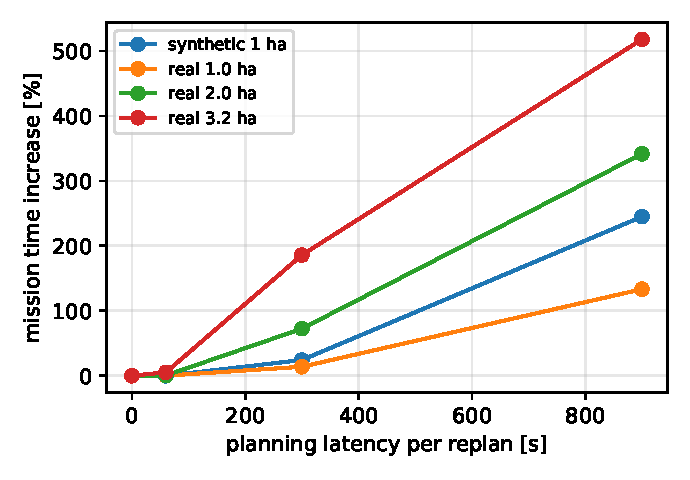
\includegraphics[width=0.62\textwidth]{figs/fig_latency.pdf}
\caption{Her yeniden planlamaya sabit bir gecikme eklendiğinde görev süresindeki artış
(Tall Spindle bahçeleri, ilk ve seyrek toplama geçişi, beş tohum)}\label{fig:latency}
\end{figure}

Sıralı bahçelerde (tüm sonuçlar: \nameref{app:rows}) PSB-MT/R, görevleri
sıra bantlarına göre ortalama \HvRowblockRelMean\% (koşuların
\HvWinRowblock\% kadarında daha hızlı), açgözlü dağıtıma göre
\HvGreedyRelMean\% (\HvWinGreedy\%) ve yeniden planlama yapmayan aynı planlayıcıya
göre \HvStaticRelMean\% (\HvWinStatic\%) kısaltmıştır. Kümelenmiş analizde sıra
bantlarına göre süre farkı $\HqRowsRowblockTime$\% iken olgun meyve/saat farkı
$\HqRowsRowblockThroughput$\% olmuştur; süre farkının güven aralığı sıfırı kapsamaktadır.
Yeniden planlama başına 1\,s süre verilen OR-Tools'un görevleri \HvOrtoolsOneRelMean\%
daha uzun sürmüş (PSB-MT/R, koşuların \HvWinOrtoolsOne\% kadarında daha hızlı);
kümelenmiş süre ve verimlilik farkları $\HqRowsOrtoolsOneTime$\% ve
$\HqRowsOrtoolsOneThroughput$\% olmuştur. Yeniden planlama başına 10\,s verildiğinde OR-Tools,
1\,ha'lık iki bahçede PSB-MT/R ile benzer ortalama sonuç vermiş (\HvOrtoolsOneZeroRelMean\%),
ancak bunu on kat planlama süresiyle sağlamıştır.

\paragraph{Planlama gecikmesi} Bir platform kasa değişimi için ortalama
\HvReplanGapMin{} dakikada bir dönmüş (koşular üzerinden medyan) ve her dönüş bir yeniden planlamayı tetiklemiştir.
Şekil~\ref{fig:latency}'de her PSB-MT/R planına yapay bir gecikme eklenmiştir. Bir dakikaya kadar
olan gecikmeler en fazla yüzde birkaçlık bir kayba yol açmış, ancak gecikme dönüşler arasındaki
aralığı aştığında planlar kuyrukta birikmiş ve görev süreleri hızla artmıştır (3.2\,ha'lık bahçede
300\,s gecikme için \HvLatOsmThreehaThreeZeroZero\%). PSB-MT/R'nin plan başına hesaplama süresi \HvPsbPlanMs\,ms olmuştur.

\subsection{Görselleştirme}
Benzetim kayıtları üç boyutlu bir Blender sahnesinde görsel olarak yeniden oynatılmıştır
(Şekil~\ref{fig:blender}): ağaç konumları, çeşitler, ağaç başına meyve sayıları,
platform yolları ve durakları, her durakta toplanan meyveler ve bölgeler kayıttan alınmış;
ağaç, elma, platform ve drone modelleri ise temsilî niteliktedir
(CC0 fotogrametri varlıkları ve gerçek ölçekte prosedürel modeller). Aynı sahne
üreteciyle eksiksiz bir görevin açıklayıcı bir videosu da üretilmiştir.

\section{Tartışma}\label{sec:discussion}

\paragraph{Hangi durumda hangi çözücü} PSB, hedeflerin sırasını onları robotlara atamadan önce
sabitlemekte, ardından optimal bölme rotaları eşik sınaması başına $O(nk)$ sürede dengelemektedir;
kurulum maliyeti $n$ ile neredeyse doğrusal olarak artmakta ve ilk çözüm saniyenin küçük bir
kesrinde elde edilmektedir. Literatürde öne çıkan
metasezgiseller ve LKH-3 çok daha geniş bir çözüm uzayını taramakta ve yeterli süre verildiğinde
daha iyi çözümler bulmaktadır; özellikle MILS, küçük örneklerde birkaç on saniye, orta büyüklükteki
örneklerde ise yaklaşık iki dakika sonra PSB+LNS'yi geçmiştir. Saniyeler içinde tamamlanması
gereken planlamada, binlerce hedef içeren örneklerde ve daha uzun bir aramaya başlangıç
çözümü sağlamak için PSB daha uygun bir seçenektir; birkaç dakikalık sürenin bulunduğu orta büyüklükteki örneklerin
çevrimdışı planlanmasında ise MILS daha uygundur.

\paragraph{Bahçede önemli olan} Hasat benzetiminde görev süresinin büyük kısmını toplama süresi oluşturmaktadır;
bu nedenle rotalama farkları görev süresine yüzde birkaçtan yaklaşık yüzde ona kadar uzanan
farklar olarak yansımaktadır. En büyük etkiler, çözücünün arama gücünden bağımsız üç karardan
kaynaklanmaktadır: toplama geçişi sırasında ortaya çıkan meyve sayılarıyla yeniden planlama,
bahçenin kendi ekseninde planlama (PSB için yaklaşık 12\%) ve planlama süresinin kasa
değişimleri arasındaki aralığın altında tutulması. PSB, plan başına milisaniyeler düzeyindeki süresiyle son
koşulu sağlamaktadır; 1\,s süre sınırıyla çalışan OR-Tools PSB'ye 2--3\% yaklaşmış, 10\,s sınırla ise
1\,ha'lık bahçelerde PSB ile benzer ortalama sonuç vermiştir. Uç devralmalı merkezi olmayan $k$-d
bölüntüsü, merkezi yeniden planlamanın mümkün olmadığı durumlarda pratik bir alternatiftir
ve devralma, bu yaklaşımın kaybının önemli bir kısmını telafi etmektedir.

\paragraph{Sınırlılıklar} (i) Hasat sonuçları benzetimden elde edilmiştir; saha denemesi
yapılmamıştır ve kablolu platform parametreleri sektör basınındaki tanımlamalara dayanan
varsayımlardır. Duyarlılık analizi yalnızca Tablo~\ref{tab:params}'de aralık verilen
parametreleri kapsar; durma/dönüş süresi gibi diğer varsayımlar ayrıca sınanmamıştır.
(ii) Algılama, görüntüler üzerinde bir dedektör çalıştırılarak değil, istatistiksel olarak
(yakalama oranı, kesinlik, görünür pay) modellenmiştir. (iii) Platformlar arasındaki etkileşimler
modellenmemiştir (çarpışma ve kablo kısıtı yoktur, kasa istasyonu kapasitesi sınırsızdır) ve
hareket, bahçe ekseninde $L_1$ uzaklıklarıyla yaklaşık olarak hesaplanmıştır; bölgede yaygın olan,
farklı yönelimli birden çok küçük parselden oluşan işletmeler ayrıca modellenmemiştir.
(iv) Literatürde öne çıkan kodlar tek bir tohum ve varsayılan parametrelerle çalıştırılmış,
bunlardan ikisi yalnızca yürütülebilir dosya olarak kullanılabilmiştir; MA en büyük örnekte
çalıştırılamamıştır. Ortak \emph{best} referansı farklı sayıda tohum içeren yöntemlerin en
iyisinden hesaplandığından sapmalar tanımlayıcıdır; 20 eşzamanlı koşunun 12 fiziksel
çekirdekteki bellek ve zaman paylaşımı etkileri ayrıca izole edilmemiştir.
(v) Alt sınır ara $k$ değerleri için zayıftır; bu nedenle bahçelerdeki mutlak kalite yalnızca
yaklaşık olarak bilinmektedir. (vi) Yöntemler eşit hasat miktarında durdurulmamıştır; bu
nedenle süre, olgun meyve payı ve verimlilik birlikte değerlendirilmelidir. Kümelenmiş
güven aralıkları yalnızca 8--10 bahçe--geçiş kümesine dayanır. (vii) Görselleştirme,
benzetimin yeniden oynatımıdır; bir uçuş testi değildir.

\section{Sonuç}\label{sec:conclusion}

Optimal min--maks bölme içeren ve önce rota, sonra küme yaklaşımına dayanan bir işlem hattı olan PSB, on bin
hedefli örnekler için saniyenin küçük bir kesrinde çözüm döndürmüş; her an sonuç veren
LNS ile birlikte de sekiz yöntem arasında $n\ge 1000$ olan örneklerde ilk saniyeler boyunca,
$n\ge 5000$ olan örneklerde ise bütçenin tamamı boyunca en düşük medyan sapmayı vermiştir.
Orta büyüklükteki örneklerde ise dakikalar mertebesinde süre bulunduğunda MILS daha iyi sonuç vermiştir. Kablolu drone
platformlarıyla seçmeli elma hasadının benzetiminde, ağaç konumlarından kestirilen bahçe
ekseninde PSB-MT/R ile yeniden planlama, sabit sıra bantlarına dayalı statik referansa kıyasla
koşuların \HgFirstRowblockWin\% kadarında ilk toplama geçişini kısaltmış ve olgun meyvenin
daha büyük bir kısmının hasat edilmesini sağlamıştır; bunun yerine harita eksenlerinde planlama
yapıldığında görevler yaklaşık 12\% uzamıştır. Gelecek çalışmalarda platformlar arası etkileşimin,
görüntü tabanlı algılamanın, serbest uçan drone'lar için batarya ve kablo kısıtlarının ele alınması ve
saha doğrulaması planlanmaktadır.


\section{Beyanlar}
\paragraph{Finansman} Bu çalışma için herhangi bir finansman alınmamıştır.

\paragraph{Çıkar çatışması} Bu makalenin içeriğiyle ilgili beyan edilecek
bir çıkar çatışması bulunmamaktadır.

\paragraph{Yazar katkıları} Ufuk Asil: kavramsallaştırma, yöntem, yazılım, biçimsel
analiz, araştırma, görselleştirme, yazım -- ilk taslak, yazım -- gözden geçirme ve
düzenleme.

\paragraph{Veri erişilebilirliği} Örnekler, deneylerin koşu düzeyindeki ham
kayıtları ve bu makaledeki sayıları, tabloları ve şekilleri üreten betikler
\url{https://github.com/ufukasia/psb-precision-agriculture} adresindeki açık depoda
sunulmaktadır; materyal kabulün ardından kalıcı bir Zenodo DOI ile arşivlenecektir.
Bahçe sınırları OpenStreetMap verilerinden türetilmiştir (\copyright{} OpenStreetMap
katkıcıları, ODbL).

\paragraph{Kod erişilebilirliği} PSB uygulaması, LKH-3 3.0.13 ve diğer çözücülerin
sarmalayıcıları, benzetimler ve Blender sahne üreteci aynı depoda MIT lisansıyla
paylaşılmaktadır; üçüncü taraf çözücüler kendi lisanslarına tabidir. Benzetilen bir
görevin açıklayıcı videosu Çevrimiçi Kaynak~1 olarak sunulmakta ve
\url{https://github.com/ufukasia/psb-precision-agriculture/releases/download/v1.0.0/ESM_1.mp4}
adresinden erişilebilmektedir.

\appendix
\section{Ek A: Literatür kümesinde örnek bazında sonuçlar}\label{app:lit}
{\tiny
\setlength{\tabcolsep}{2.6pt}
\begin{longtable}{l*{11}{r}}
\caption{Literatür örnekleri: referans değere göre sapma (\%; referans, yayımlanmış
BKS ile \citet{hehaoxia2024} sonuçlarının en iyisidir). PSB tek atış sütunu yalnızca kurulum
adımını gösterir; diğer sütunlar nihai değerlerdir (PSB: PSB+LNS; PSB+LNS ve LKH-3 için
tohumlar üzerinden medyan); ``nihai'', bütçe sonundaki değeri ifade eder ($n<1000$ için 120\,s,
$n<5000$ için 300\,s, aksi halde 600\,s). Kalın: en iyi nihai değer}\label{tab:lit}\\
\rawinput{tab_lit.tex}
\end{longtable}}

\clearpage
\section{Ek B: Tall Spindle sıralı bahçeler}\label{app:rows}
{\scriptsize
\setlength{\tabcolsep}{4pt}
\begin{longtable}{lrrrrr}
\caption{Tall Spindle bahçeler: beş tohum üzerinden ortalama görev süresi, PSB-MT/R'ye
göre göreli fark, toplanan olgun meyve payı, platform süresinde yolun payı ve görev
başına toplam planlama süresi}\label{tab:rows}\\
\rawinput{tab_harvest.tex}
\end{longtable}}

\clearpage
\bibliographystyle{plainnat}
\bibliography{refs}
\end{document}
